\documentclass[aspectratio=169, 11pt]{beamer}

\usetheme{Madrid}
\usecolortheme{whale}
\setbeamercolor{frametitle}{bg=blue!8, fg=black}
\setbeamercolor{title}{bg=blue!12, fg=black}
\setbeamercolor{structure}{fg=blue!50!black}
\setbeamercolor{item}{fg=blue!50!black}
\setbeamertemplate{navigation symbols}{}
\setbeamertemplate{footline}{
  \leavevmode\hbox{%
    \begin{beamercolorbox}[wd=.35\paperwidth,ht=2.5ex,dp=1ex,left]{author in head/foot}%
      \hspace*{1em}\footnotesize Machine Learning with R (Dr.\ Endri Ra\c{c}o)
    \end{beamercolorbox}%
    \begin{beamercolorbox}[wd=.35\paperwidth,ht=2.5ex,dp=1ex,center]{title in head/foot}%
      \footnotesize Resampling Methods
    \end{beamercolorbox}%
    \begin{beamercolorbox}[wd=.3\paperwidth,ht=2.5ex,dp=1ex,right]{date in head/foot}%
      \footnotesize Week 3, 2025 \hspace*{1em} \insertframenumber{} / \inserttotalframenumber \hspace*{1em}
    \end{beamercolorbox}}%
}

\usepackage{amsmath,amssymb,mathtools}
\usepackage{tikz}
\usetikzlibrary{arrows.meta, positioning, calc, shapes, decorations.pathreplacing, patterns}
\usepackage{pgfplots}
\pgfplotsset{compat=1.18}
\usepackage{booktabs}
\usepackage{xcolor}

\definecolor{accent}{RGB}{59,130,246}
\definecolor{darkblue}{RGB}{30,39,97}
\definecolor{softred}{RGB}{239,68,68}
\definecolor{softgreen}{RGB}{16,185,129}
\definecolor{amber}{RGB}{245,158,11}
\definecolor{muted}{RGB}{100,116,139}
\definecolor{orange}{RGB}{249,115,22}
\definecolor{beige}{RGB}{245,235,210}

\title{Resampling Methods}
\subtitle{Cross-Validation \& Bootstrap --- ISLR Chapter 5}
\author{Machine Learning with R}
\institute{Dr.\ Endri Ra\c{c}o}
\date{Week 3, 2025}

\begin{document}

\begin{frame}
\titlepage
\end{frame}


\begin{frame}{The Central Question}
\begin{columns}
\column{0.5\textwidth}
\textbf{Weeks 1--2:} We fit models

\textbf{Today:} How good are they \textit{really}?

\vspace{0.5em}
\textbf{Two problems:}

\begin{enumerate}
  \item \textbf{Model assessment:}\\How well does the model predict new data?
  \item \textbf{Model selection:}\\Which model (or tuning parameter) is best?
\end{enumerate}

\vspace{0.3em}
Both require estimating \textbf{test error}

\column{0.45\textwidth}
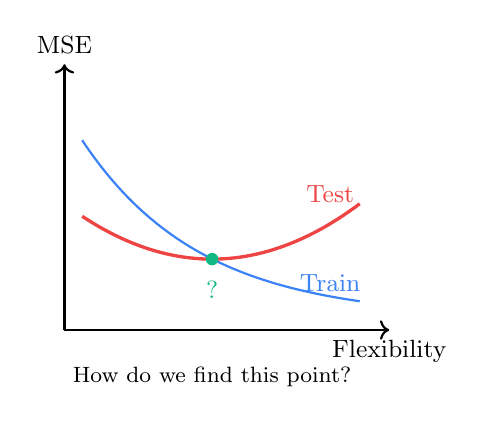
\begin{tikzpicture}[scale=0.75]
  \draw[->, thick] (0,0) -- (5.5,0) node[below] {\small Flexibility};
  \draw[->, thick] (0,0) -- (0,4.5) node[above] {\small MSE};
  \draw[accent, thick, domain=0.3:5, samples=50] plot (\x, {3.5*exp(-0.5*\x)+0.2});
  \node[accent] at (4.5, 0.8) {\small Train};
  \draw[softred, very thick, domain=0.3:5, samples=50] plot (\x, {0.15*(\x-2.5)*(\x-2.5)+1.2});
  \node[softred] at (4.5, 2.3) {\small Test};
  \fill[softgreen] (2.5, 1.2) circle (3pt);
  \node[softgreen, below] at (2.5, 1.0) {\small ?};
  \node at (2.5, -0.8) {\footnotesize How do we find this point?};
\end{tikzpicture}
\end{columns}
\end{frame}


\begin{frame}{Why Not Use Training Error?}
\begin{columns}
\column{0.55\textwidth}
$\text{Training MSE} = \frac{1}{n}\sum_{i=1}^n (y_i - \hat{f}(x_i))^2$

\vspace{0.5em}
\textbf{Problem:}

Training MSE \textbf{always} decreases with flexibility

It can even reach \textbf{zero} (overfitting!)

\vspace{0.3em}
Low training error $\neq$ good prediction

\vspace{0.5em}
\textbf{What we need:}

Test error on \textbf{new, unseen data}

\vspace{0.3em}
But we usually don't have a test set!

\column{0.4\textwidth}
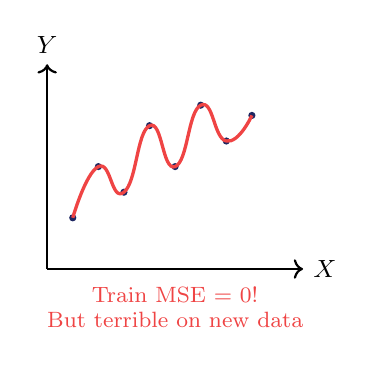
\begin{tikzpicture}[scale=0.65]
  \draw[->, thick] (0,0) -- (5,0) node[right] {\small $X$};
  \draw[->, thick] (0,0) -- (0,4) node[above] {\small $Y$};
  \foreach \x/\y in {0.5/1, 1/2, 1.5/1.5, 2/2.8, 2.5/2, 3/3.2, 3.5/2.5, 4/3} {
    \fill[darkblue] (\x, \y) circle (2pt);
  }
  \draw[softred, very thick, smooth, tension=0.9] plot coordinates {(0.5,1)(1,2)(1.5,1.5)(2,2.8)(2.5,2)(3,3.2)(3.5,2.5)(4,3)};
  \node[softred] at (2.5, -0.5) {\footnotesize Train MSE = 0!};
  \node[softred] at (2.5, -1) {\footnotesize But terrible on new data};
\end{tikzpicture}

\vspace{0.3em}
\textcolor{accent}{\textbf{Solution: Resampling}}
\end{columns}
\end{frame}


\begin{frame}{Today's Roadmap}
\begin{columns}
\column{0.48\textwidth}
\textbf{Cross-Validation:}
\begin{enumerate}
  \item Validation Set Approach
  \item Leave-One-Out CV (LOOCV)
  \item $k$-Fold CV
  \item Bias-Variance trade-off for $k$
\end{enumerate}

\column{0.48\textwidth}
\textbf{Bootstrap:}
\begin{enumerate}
  \setcounter{enumi}{4}
  \item The bootstrap idea
  \item Estimating uncertainty
  \item Bootstrap for regression
\end{enumerate}

\vspace{0.5em}
\textbf{Datasets:}

\texttt{Auto}, \texttt{Default}, \texttt{Portfolio}
\end{columns}
\end{frame}


% ═══════════ VALIDATION SET APPROACH ═══════════
\begin{frame}{Approach 1: The Validation Set}
\begin{columns}
\column{0.55\textwidth}
\textbf{Simplest idea:}

\begin{enumerate}
  \item Randomly split data into two halves
  \item Train on one half
  \item Evaluate on the other half
\end{enumerate}

\vspace{0.5em}
\textbf{Example:} Auto data, $n = 392$

Split: 196 train, 196 test

Fit: $\texttt{mpg} \sim \texttt{poly(horsepower, d)}$

Compute test MSE for $d = 1, 2, \ldots, 10$

\column{0.4\textwidth}
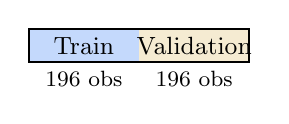
\begin{tikzpicture}[scale=0.7]
  % Data bar
  \fill[accent!30] (0, 0) rectangle (2, 0.6);
  \fill[beige] (2, 0) rectangle (4, 0.6);
  \draw[thick] (0,0) rectangle (4, 0.6);
  \node[font=\small] at (1, 0.3) {Train};
  \node[font=\small] at (3, 0.3) {Validation};
  \node[font=\footnotesize] at (1, -0.3) {196 obs};
  \node[font=\footnotesize] at (3, -0.3) {196 obs};
\end{tikzpicture}

\vspace{1em}
\textbf{Problems:}
\begin{itemize}
  \item High \textbf{variance}: different splits $\Rightarrow$ different MSEs
  \item Only half the data for training $\Rightarrow$ \textbf{overestimates} test error
\end{itemize}
\end{columns}
\end{frame}


\begin{frame}{Validation Set: The Variance Problem}
\begin{columns}
\column{0.55\textwidth}
\textbf{10 different random splits:}

Each gives a different test MSE curve!

\vspace{0.3em}
The \textbf{minimum} varies: sometimes $d=2$, sometimes $d=5$

\vspace{0.3em}
This is \textbf{unreliable} for model selection

\vspace{0.5em}
\textbf{Root cause:}

With only $n/2$ training points, the model has high variance

Results are too dependent on which observations end up in which half

\column{0.4\textwidth}
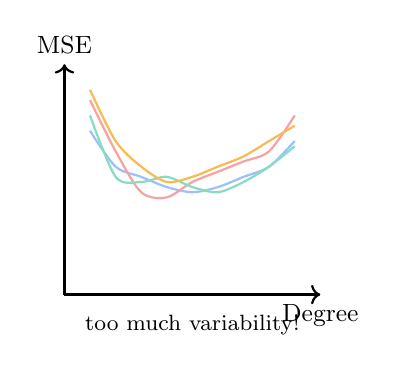
\begin{tikzpicture}[scale=0.65]
  \draw[->, thick] (0,0) -- (5,0) node[below] {\small Degree};
  \draw[->, thick] (0,0) -- (0,4.5) node[above] {\small MSE};
  % Multiple curves (different splits)
  \draw[accent!50, thick, smooth] plot coordinates {(0.5,3.2)(1,2.5)(1.5,2.3)(2,2.1)(2.5,2.0)(3,2.1)(3.5,2.3)(4,2.5)(4.5,3.0)};
  \draw[softred!50, thick, smooth] plot coordinates {(0.5,3.8)(1,2.8)(1.5,2.0)(2,1.9)(2.5,2.2)(3,2.4)(3.5,2.6)(4,2.8)(4.5,3.5)};
  \draw[softgreen!50, thick, smooth] plot coordinates {(0.5,3.5)(1,2.3)(1.5,2.2)(2,2.3)(2.5,2.1)(3,2.0)(3.5,2.2)(4,2.5)(4.5,2.9)};
  \draw[amber!70, thick, smooth] plot coordinates {(0.5,4.0)(1,3.0)(1.5,2.5)(2,2.2)(2.5,2.3)(3,2.5)(3.5,2.7)(4,3.0)(4.5,3.3)};
  \node at (2.5, -0.6) {\footnotesize too much variability!};
\end{tikzpicture}

\vspace{0.5em}
\textcolor{accent}{\textbf{Solution: Use more of the data}}
\end{columns}
\end{frame}


% ═══════════ LOOCV ═══════════
\begin{frame}{Approach 2: Leave-One-Out CV (LOOCV)}

\textbf{Idea:} Train on $n-1$ observations, test on the 1 left out. Repeat $n$ times.

\vspace{0.3em}
\begin{center}
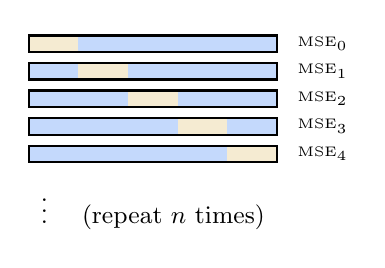
\begin{tikzpicture}[scale=0.7]
  \foreach \i in {0,...,4} {
    \fill[accent!30] (0, {2-\i*0.5}) rectangle (4.5, {2.3-\i*0.5});
    \fill[beige] ({\i*0.9}, {2-\i*0.5}) rectangle ({(\i+1)*0.9}, {2.3-\i*0.5});
    \draw[thick] (0, {2-\i*0.5}) rectangle (4.5, {2.3-\i*0.5});
    \node[font=\tiny, right] at (4.7, {2.15-\i*0.5}) {$\text{MSE}_{\pgfmathprintnumber{\i}}$};
  }
  \node[font=\small] at (2.25, -0.8) {$\vdots$ \quad (repeat $n$ times)};
\end{tikzpicture}
\end{center}

$$\text{CV}_{(n)} = \frac{1}{n}\sum_{i=1}^{n} \text{MSE}_i = \frac{1}{n}\sum_{i=1}^{n}(y_i - \hat{y}_i^{(-i)})^2$$

where $\hat{y}_i^{(-i)}$ = prediction for $i$ from model trained \textbf{without} observation $i$
\end{frame}


\begin{frame}{LOOCV: Pros, Cons, and a Shortcut}
\begin{columns}
\column{0.48\textwidth}
\textbf{Advantages:}
\begin{itemize}
  \item[\textcolor{softgreen}{\textbullet}] Nearly unbiased (trains on $n-1$)
  \item[\textcolor{softgreen}{\textbullet}] No randomness in the split
  \item[\textcolor{softgreen}{\textbullet}] Uses almost all data for training
\end{itemize}

\vspace{0.3em}
\textbf{Disadvantages:}
\begin{itemize}
  \item[\textcolor{softred}{\textbullet}] Expensive: fit model $n$ times
  \item[\textcolor{softred}{\textbullet}] High variance (correlated estimates)
\end{itemize}

\column{0.48\textwidth}
\textbf{Magic shortcut} (linear models only!):

$$\text{CV}_{(n)} = \frac{1}{n}\sum_{i=1}^{n}\left(\frac{y_i - \hat{y}_i}{1 - h_i}\right)^2$$

where $h_i$ = leverage of observation $i$

\vspace{0.3em}
\textcolor{softgreen}{Requires fitting the model only \textbf{once}!}

\vspace{0.3em}
Inflates residuals for high-leverage points by exactly the right amount
\end{columns}
\end{frame}


\begin{frame}{LOOCV: Worked Example on Auto}

\textbf{Fit:} $\texttt{mpg} \sim \texttt{poly(horsepower}, d)$ for $d = 1, \ldots, 10$

\vspace{0.3em}
\begin{columns}
\column{0.45\textwidth}
\begin{tabular}{cc}
\toprule
Degree $d$ & LOOCV MSE \\
\midrule
1 & 24.23 \\
\textcolor{softgreen}{2} & \textcolor{softgreen}{19.25} \\
3 & 19.33 \\
4 & 19.42 \\
5 & 19.03 \\
\bottomrule
\end{tabular}

\vspace{0.3em}
\textbf{Sharp drop} from linear to quadratic!

No clear gain beyond $d = 2$

\column{0.5\textwidth}
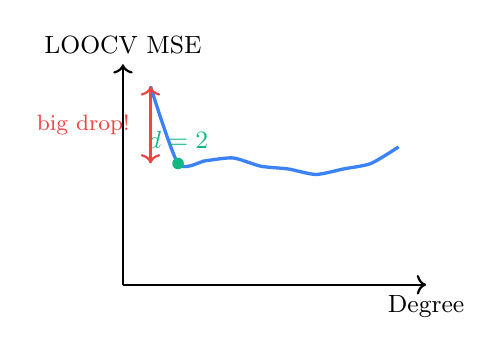
\begin{tikzpicture}[scale=0.7]
  \draw[->, thick] (0,0) -- (5.5,0) node[below] {\small Degree};
  \draw[->, thick] (0,0) -- (0,4) node[above] {\small LOOCV MSE};
  % LOOCV curve
  \draw[accent, very thick, smooth, tension=0.4] plot coordinates {(0.5,3.6)(1,2.2)(1.5,2.25)(2,2.3)(2.5,2.15)(3,2.1)(3.5,2.0)(4,2.1)(4.5,2.2)(5,2.5)};
  \fill[softgreen] (1, 2.2) circle (3pt);
  \node[softgreen, above] at (1, 2.3) {\small $d=2$};
  % Drop annotation
  \draw[softred, thick, <->] (0.5, 3.6) -- (0.5, 2.2);
  \node[softred, left, font=\footnotesize] at (0.3, 2.9) {big drop!};
\end{tikzpicture}

\vspace{0.3em}
\footnotesize R: \texttt{cv.glm(Auto, glm.fit)\$delta[1]}
\end{columns}
\end{frame}


% ═══════════ K-FOLD CV ═══════════
\begin{frame}{Approach 3: $k$-Fold Cross-Validation}
\begin{columns}
\column{0.55\textwidth}
\textbf{Split data into $k$ equal folds}

\begin{enumerate}
  \item Hold out fold 1 $\Rightarrow$ test; train on folds 2--$k$
  \item Hold out fold 2 $\Rightarrow$ test; train on rest
  \item[] $\vdots$
  \item[$k$.] Hold out fold $k$ $\Rightarrow$ test; train on rest
\end{enumerate}

$$\text{CV}_{(k)} = \frac{1}{k}\sum_{i=1}^{k}\text{MSE}_i$$

Typical: $k = 5$ or $k = 10$

LOOCV = special case where $k = n$

\column{0.4\textwidth}
\textbf{5-fold CV:}

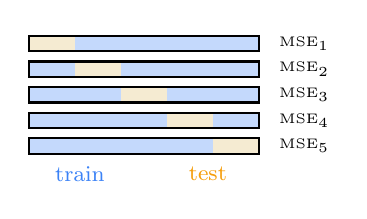
\begin{tikzpicture}[scale=0.65]
  % Fold 1
  \fill[beige] (0, 2.2) rectangle (0.9, 2.5);
  \fill[accent!30] (0.9, 2.2) rectangle (4.5, 2.5);
  \draw[thick] (0, 2.2) rectangle (4.5, 2.5);
  \node[font=\tiny, right] at (4.7, 2.35) {MSE$_1$};
  % Fold 2
  \fill[accent!30] (0, 1.7) rectangle (0.9, 2.0);
  \fill[beige] (0.9, 1.7) rectangle (1.8, 2.0);
  \fill[accent!30] (1.8, 1.7) rectangle (4.5, 2.0);
  \draw[thick] (0, 1.7) rectangle (4.5, 2.0);
  \node[font=\tiny, right] at (4.7, 1.85) {MSE$_2$};
  % Fold 3
  \fill[accent!30] (0, 1.2) rectangle (1.8, 1.5);
  \fill[beige] (1.8, 1.2) rectangle (2.7, 1.5);
  \fill[accent!30] (2.7, 1.2) rectangle (4.5, 1.5);
  \draw[thick] (0, 1.2) rectangle (4.5, 1.5);
  \node[font=\tiny, right] at (4.7, 1.35) {MSE$_3$};
  % Fold 4
  \fill[accent!30] (0, 0.7) rectangle (2.7, 1.0);
  \fill[beige] (2.7, 0.7) rectangle (3.6, 1.0);
  \fill[accent!30] (3.6, 0.7) rectangle (4.5, 1.0);
  \draw[thick] (0, 0.7) rectangle (4.5, 1.0);
  \node[font=\tiny, right] at (4.7, 0.85) {MSE$_4$};
  % Fold 5
  \fill[accent!30] (0, 0.2) rectangle (3.6, 0.5);
  \fill[beige] (3.6, 0.2) rectangle (4.5, 0.5);
  \draw[thick] (0, 0.2) rectangle (4.5, 0.5);
  \node[font=\tiny, right] at (4.7, 0.35) {MSE$_5$};
  % Legend
  \node[accent, font=\footnotesize] at (1, -0.2) {train};
  \node[font=\footnotesize] at (3.5, -0.2) {\textcolor{amber}{test}};
\end{tikzpicture}

\vspace{0.5em}
\textcolor{softgreen}{Only fit model $k$ times!}\\
\footnotesize (vs.\ $n$ times for LOOCV)
\end{columns}
\end{frame}


\begin{frame}{$k$-Fold CV: The Bias-Variance Trade-Off}

\begin{center}
\begin{tabular}{lccc}
\toprule
Method & Bias & Variance & Computation \\
\midrule
Validation set ($k=2$) & \textcolor{softred}{High} & \textcolor{softred}{High} & \textcolor{softgreen}{Fast} \\
5-fold CV & Medium & \textcolor{softgreen}{Low} & \textcolor{softgreen}{Fast} \\
10-fold CV & Low & \textcolor{softgreen}{Low} & Medium \\
LOOCV ($k=n$) & \textcolor{softgreen}{Very low} & \textcolor{softred}{High} & \textcolor{softred}{Slow} \\
\bottomrule
\end{tabular}
\end{center}

\vspace{0.5em}
\begin{columns}
\column{0.55\textwidth}
\textbf{Why does LOOCV have high variance?}

\vspace{0.2em}
We average $n$ estimates, each trained on \textbf{nearly identical} data

$\Rightarrow$ Estimates are highly \textbf{correlated}

$\Rightarrow$ Averaging correlated quantities reduces variance less

\column{0.4\textwidth}
\textbf{Why does $k=5$ have more bias?}

\vspace{0.2em}
Each fold trains on $(k-1)/k$ of data

$k=5$: trains on 80\%

$k=n$: trains on $\approx 100\%$

\vspace{0.3em}
\textcolor{accent}{\textbf{Sweet spot: $k = 5$ or $k = 10$}}
\end{columns}
\end{frame}


\begin{frame}{Why $k = 10$? A Visual Argument}

\begin{center}
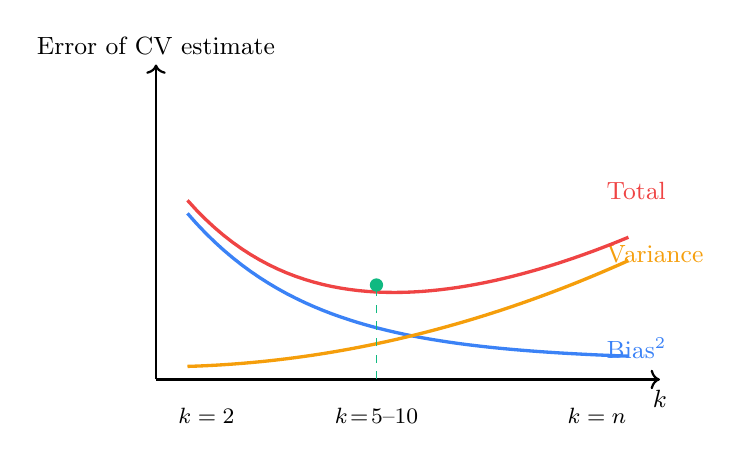
\begin{tikzpicture}[scale=0.8]
  \draw[->, thick] (0,0) -- (8,0) node[below] {\small $k$};
  \draw[->, thick] (0,0) -- (0,5) node[above] {\small Error of CV estimate};

  % Bias (decreasing)
  \draw[accent, very thick, domain=0.5:7.5, samples=50] plot (\x, {3*exp(-0.5*\x)+0.3});
  \node[accent, right] at (7, 0.5) {\small Bias$^2$};

  % Variance (increasing)
  \draw[amber, very thick, domain=0.5:7.5, samples=50] plot (\x, {0.03*\x*\x + 0.2});
  \node[amber, right] at (7, 2.0) {\small Variance};

  % Total
  \draw[softred, very thick, domain=0.5:7.5, samples=50] plot (\x, {3*exp(-0.5*\x) + 0.03*\x*\x + 0.5});
  \node[softred, right] at (7, 3.0) {\small Total};

  % Sweet spot
  \draw[softgreen, dashed] (3.5, 0) -- (3.5, 1.5);
  \fill[softgreen] (3.5, 1.5) circle (3pt);

  % Labels
  \node[below] at (0.8, -0.3) {\footnotesize $k=2$};
  \node[below] at (3.5, -0.3) {\footnotesize $k\!=\!5$--$10$};
  \node[below] at (7, -0.3) {\footnotesize $k=n$};
\end{tikzpicture}
\end{center}

Empirically, $k = 5$ or $k = 10$ gives the best bias-variance balance
\end{frame}


\begin{frame}{CV for Classification}

Same idea, but use \textbf{error rate} instead of MSE:

$$\text{CV}_{(k)} = \frac{1}{k}\sum_{i=1}^{k}\text{Err}_i \qquad \text{where } \text{Err}_i = \frac{1}{n_i}\sum_{j \in C_i} \mathbf{1}(y_j \neq \hat{y}_j)$$

\begin{columns}
\column{0.5\textwidth}
\textbf{Example: Logistic on Default}

\vspace{0.3em}
\begin{tabular}{cc}
\toprule
Method & CV Error \\
\midrule
Validation set & 2.7\% \\
LOOCV & 2.6\% \\
10-fold CV & 2.6\% \\
\bottomrule
\end{tabular}

\vspace{0.3em}
All give similar results here

\column{0.45\textwidth}
\textbf{CV for model selection:}

Which polynomial degree for logistic?

\vspace{0.3em}
\begin{enumerate}
  \item For each $d = 1, \ldots, 5$:
  \item[] \quad Compute 10-fold CV error
  \item Pick $d$ with lowest CV error
  \item Refit on full data with that $d$
\end{enumerate}
\end{columns}
\end{frame}


\begin{frame}{CV in Practice: The Complete Workflow}

\begin{center}
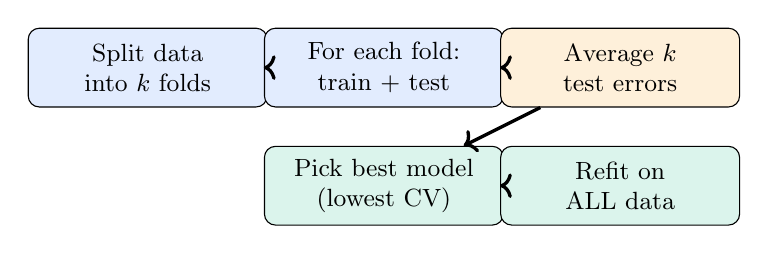
\begin{tikzpicture}[scale=0.75, every node/.style={font=\small, text width=2.8cm, align=center}]
  \node[draw, fill=accent!15, rounded corners, minimum height=1cm] (split) at (0,0) {Split data into $k$ folds};
  \node[draw, fill=accent!15, rounded corners, minimum height=1cm] (loop) at (4,0) {For each fold:\\train + test};
  \node[draw, fill=amber!15, rounded corners, minimum height=1cm] (avg) at (8,0) {Average $k$\\test errors};
  \node[draw, fill=softgreen!15, rounded corners, minimum height=1cm] (pick) at (4,-2) {Pick best model\\(lowest CV)};
  \node[draw, fill=softgreen!15, rounded corners, minimum height=1cm] (refit) at (8,-2) {Refit on\\ALL data};

  \draw[->, very thick] (split) -- (loop);
  \draw[->, very thick] (loop) -- (avg);
  \draw[->, very thick] (avg) -- (pick);
  \draw[->, very thick] (pick) -- (refit);
\end{tikzpicture}
\end{center}

\vspace{0.5em}
\textbf{Important:} After selecting the best model via CV, \textbf{refit} it on the entire dataset to get the final model!
\end{frame}


% ═══════════ BOOTSTRAP ═══════════
\begin{frame}{The Bootstrap: A Completely Different Idea}
\begin{columns}
\column{0.55\textwidth}
\textbf{Problem:}

How variable is our estimate $\hat{\theta}$?

\vspace{0.3em}
\textit{``If I collected data again, how different would $\hat{\theta}$ be?''}

\vspace{0.5em}
\textbf{Ideal (impossible):}

Collect 1000 new datasets from the population, compute $\hat{\theta}$ each time

\vspace{0.5em}
\textbf{Bootstrap (practical):}

Sample \textbf{with replacement} from our dataset,\\
pretend each resample is a new dataset

\column{0.4\textwidth}
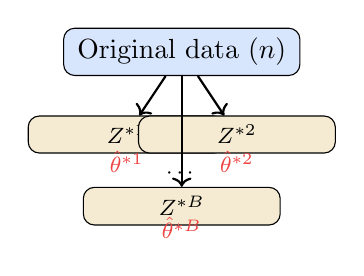
\begin{tikzpicture}[scale=0.7]
  % Original
  \node[draw, fill=accent!20, rounded corners, minimum width=3cm, minimum height=0.6cm] (orig) at (0, 3) {Original data ($n$)};
  % Bootstrap samples
  \node[draw, fill=beige, rounded corners, minimum width=2.5cm, minimum height=0.4cm, font=\footnotesize] (b1) at (-1, 1.5) {$Z^{*1}$};
  \node[draw, fill=beige, rounded corners, minimum width=2.5cm, minimum height=0.4cm, font=\footnotesize] (b2) at (1, 1.5) {$Z^{*2}$};
  \node[font=\footnotesize] at (0, 0.8) {$\cdots$};
  \node[draw, fill=beige, rounded corners, minimum width=2.5cm, minimum height=0.4cm, font=\footnotesize] (bB) at (0, 0.2) {$Z^{*B}$};
  % Arrows
  \draw[->, thick] (orig) -- (b1);
  \draw[->, thick] (orig) -- (b2);
  \draw[->, thick] (orig) -- (bB);
  % Theta hats
  \node[font=\footnotesize, softred] at (-1, 1) {$\hat{\theta}^{*1}$};
  \node[font=\footnotesize, softred] at (1, 1) {$\hat{\theta}^{*2}$};
  \node[font=\footnotesize, softred] at (0, -0.2) {$\hat{\theta}^{*B}$};
\end{tikzpicture}
\end{columns}
\end{frame}


\begin{frame}{Bootstrap: How It Works}

\textbf{Sampling with replacement:}

\begin{columns}
\column{0.5\textwidth}
\textbf{Original data:} $\{1, 2, 3, 4, 5\}$

\vspace{0.3em}
\textbf{Bootstrap sample 1:} $\{2, 1, 4, 2, 5\}$

\textbf{Bootstrap sample 2:} $\{3, 3, 1, 5, 4\}$

\textbf{Bootstrap sample 3:} $\{5, 1, 1, 3, 2\}$

\vspace{0.3em}
Same size $n$, but with \textbf{repeats}

Some observations appear multiple times;\\
others are left out

\column{0.45\textwidth}
\textbf{On average:}

Each bootstrap sample contains $\approx 63.2\%$ of unique observations

$$P(\text{obs } j \text{ not in sample}) = \left(1 - \frac{1}{n}\right)^n \approx e^{-1} \approx 0.368$$

So $\approx 36.8\%$ are \textbf{out-of-bag} (OOB)

\vspace{0.3em}
\textit{This is useful! (more in Week 6)}
\end{columns}
\end{frame}


\begin{frame}{Bootstrap: The Algorithm}

\textbf{To estimate} $\text{SE}(\hat{\theta})$:

\vspace{0.5em}
\begin{enumerate}
  \item Repeat $B$ times ($B = 1000$ or more):
  \begin{enumerate}
    \item[a.] Draw a sample of size $n$ \textbf{with replacement} from data
    \item[b.] Compute $\hat{\theta}^{*b}$ on this bootstrap sample
  \end{enumerate}
  \item Estimate the standard error:
\end{enumerate}

$$\text{SE}_B(\hat{\theta}) = \sqrt{\frac{1}{B-1}\sum_{b=1}^{B}\left(\hat{\theta}^{*b} - \bar{\hat{\theta}}^*\right)^2}$$

where $\bar{\hat{\theta}}^* = \frac{1}{B}\sum_{b=1}^B \hat{\theta}^{*b}$

\vspace{0.3em}
\centering
\textit{The variability across bootstrap samples mimics the variability across real datasets!}
\end{frame}


\begin{frame}{Bootstrap: Worked Example --- Portfolio Allocation}
\begin{columns}
\column{0.5\textwidth}
\textbf{Two assets:} $X$ and $Y$

Invest fraction $\alpha$ in $X$, $(1-\alpha)$ in $Y$

\vspace{0.3em}
\textbf{Optimal allocation:}

$$\alpha = \frac{\sigma_Y^2 - \sigma_{XY}}{\sigma_X^2 + \sigma_Y^2 - 2\sigma_{XY}}$$

minimizes $\text{Var}(\alpha X + (1-\alpha) Y)$

\vspace{0.3em}
$\alpha$ depends on $\sigma_X^2, \sigma_Y^2, \sigma_{XY}$\\
which we estimate from data

\textbf{How variable is $\hat{\alpha}$?}

\column{0.45\textwidth}
\textbf{Bootstrap results:}

$B = 1000$ bootstrap samples

\vspace{0.3em}
$\hat{\alpha} = 0.576$

$\text{SE}_B(\hat{\alpha}) = 0.089$

\vspace{0.5em}
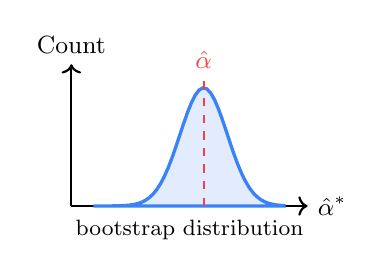
\begin{tikzpicture}[scale=0.6]
  \draw[->, thick] (0,0) -- (5,0) node[right] {\small $\hat{\alpha}^*$};
  \draw[->, thick] (0,0) -- (0,3) node[above] {\small Count};
  \draw[accent, very thick, domain=0.5:4.5, samples=50, fill=accent!15] plot (\x, {2.5*exp(-2*(\x-2.8)*(\x-2.8))}) -- (4.5,0) -- (0.5,0) -- cycle;
  \draw[softred, thick, dashed] (2.8, 0) -- (2.8, 2.7);
  \node[softred, above] at (2.8, 2.7) {\small $\hat{\alpha}$};
  \node at (2.5, -0.5) {\footnotesize bootstrap distribution};
\end{tikzpicture}
\end{columns}
\end{frame}


\begin{frame}{Bootstrap for Regression Coefficients}

\textbf{Goal:} Estimate $\text{SE}(\hat{\beta}_0)$ and $\text{SE}(\hat{\beta}_1)$ for SLR

\vspace{0.3em}
\begin{columns}
\column{0.5\textwidth}
\textbf{Formula approach (Week 1):}

$$\text{SE}(\hat{\beta}_1) = \sqrt{\frac{\sigma^2}{\sum(x_i - \bar{x})^2}}$$

Assumes: linear model, constant $\sigma^2$,\\
independent errors

\vspace{0.3em}
\textbf{Bootstrap approach:}

No assumptions needed!

\column{0.45\textwidth}
\textbf{Auto data results:}

\begin{tabular}{lcc}
\toprule
 & Formula SE & Bootstrap SE \\
\midrule
$\hat{\beta}_0$ & 0.717 & 0.860 \\
$\hat{\beta}_1$ & 0.006 & 0.007 \\
\bottomrule
\end{tabular}

\vspace{0.5em}
Bootstrap SE is \textbf{larger}!

\textit{Why? The formula assumes linearity, but the true relationship is non-linear $\Rightarrow$ formula SEs are too optimistic}
\end{columns}
\end{frame}


\begin{frame}{When Bootstrap SEs Differ from Formula SEs}
\begin{columns}
\column{0.5\textwidth}
\textbf{If assumptions hold:}

Formula SE $\approx$ Bootstrap SE

Both are valid

\vspace{0.5em}
\textbf{If assumptions are violated:}

Bootstrap SE $>$ Formula SE (usually)

\vspace{0.3em}
\textbf{Trust the bootstrap!}

It accounts for model misspecification

\column{0.45\textwidth}
\textbf{Common violations:}

\begin{itemize}
  \item Non-linearity
  \item Heteroscedasticity
  \item Correlated errors
  \item Outliers
\end{itemize}

\vspace{0.5em}
\textit{The bootstrap ``sees'' these problems;\\the formula doesn't}

\vspace{0.3em}
\fbox{\footnotesize Bootstrap = model-free uncertainty}
\end{columns}
\end{frame}


% ═══════════ DEEP DIVES ═══════════

\begin{frame}{Think About It: What Does ``Test Error'' Really Mean?}
\begin{columns}
\column{0.55\textwidth}
\textbf{Test MSE:}
$$\text{Err} = E\left[(Y - \hat{f}(X))^2\right]$$

Expectation over \textbf{new} $(X, Y)$ pairs drawn from the same population

\vspace{0.5em}
\textbf{Training MSE:}
$$\frac{1}{n}\sum_{i=1}^n (y_i - \hat{f}(x_i))^2$$

Computed on the \textbf{same data} used to build $\hat{f}$

\vspace{0.3em}
Always $\leq$ test MSE (often much less)

\column{0.4\textwidth}
\textbf{Analogy:}

\vspace{0.3em}
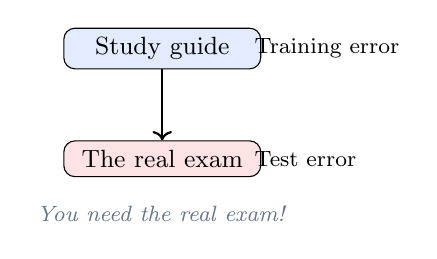
\begin{tikzpicture}[scale=0.7]
  \node[draw, fill=accent!15, rounded corners, minimum width=2.5cm, font=\small] (train) at (0,3) {Study guide};
  \node[draw, fill=softred!15, rounded corners, minimum width=2.5cm, font=\small] (test) at (0,1) {The real exam};
  \draw[->, thick] (train) -- (test);
  \node[right, font=\footnotesize] at (1.5, 3) {Training error};
  \node[right, font=\footnotesize] at (1.5, 1) {Test error};
  \node[font=\footnotesize, muted] at (0, 0) {\textit{You need the real exam!}};
\end{tikzpicture}

\vspace{0.3em}
Memorizing answers $\neq$ understanding

Overfitting $=$ memorization
\end{columns}
\end{frame}


\begin{frame}{The Resampling Toolbox: Big Picture}

\begin{center}
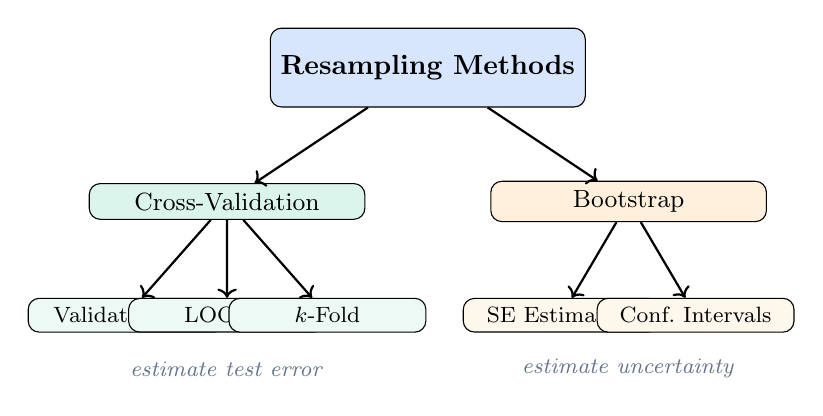
\begin{tikzpicture}[scale=0.85, every node/.style={font=\small}]
  \node[draw, fill=accent!20, rounded corners, minimum width=4cm, minimum height=1cm, font=\bfseries] (top) at (0,4) {Resampling Methods};

  \node[draw, fill=softgreen!15, rounded corners, minimum width=3.5cm] (cv) at (-3,2) {Cross-Validation};
  \node[draw, fill=amber!15, rounded corners, minimum width=3.5cm] (bs) at (3,2) {Bootstrap};

  \node[draw, fill=softgreen!8, rounded corners, font=\footnotesize, minimum width=2.5cm] (vs) at (-4.5,0.3) {Validation Set};
  \node[draw, fill=softgreen!8, rounded corners, font=\footnotesize, minimum width=2.5cm] (loo) at (-3,0.3) {LOOCV};
  \node[draw, fill=softgreen!8, rounded corners, font=\footnotesize, minimum width=2.5cm] (kf) at (-1.5,0.3) {$k$-Fold};

  \node[draw, fill=amber!8, rounded corners, font=\footnotesize, minimum width=2.5cm] (se) at (2,0.3) {SE Estimation};
  \node[draw, fill=amber!8, rounded corners, font=\footnotesize, minimum width=2.5cm] (ci) at (4,0.3) {Conf.\ Intervals};

  \draw[->, thick] (top) -- (cv);
  \draw[->, thick] (top) -- (bs);
  \draw[->, thick] (cv) -- (vs);
  \draw[->, thick] (cv) -- (loo);
  \draw[->, thick] (cv) -- (kf);
  \draw[->, thick] (bs) -- (se);
  \draw[->, thick] (bs) -- (ci);

  \node[font=\footnotesize, muted] at (-3, -0.5) {\textit{estimate test error}};
  \node[font=\footnotesize, muted] at (3, -0.5) {\textit{estimate uncertainty}};
\end{tikzpicture}
\end{center}
\end{frame}


\begin{frame}{Validation Set: Step-by-Step with Numbers}
\begin{columns}
\column{0.48\textwidth}
\textbf{Auto data:} $n = 392$

$Y$ = mpg, $X$ = horsepower

\vspace{0.3em}
\textbf{Step 1:} Split randomly

Train: obs $\{3,7,1,9,12,\ldots\}$ ($n=196$)

Test: obs $\{2,4,5,6,8,\ldots\}$ ($n=196$)

\vspace{0.3em}
\textbf{Step 2:} Fit on train only

$\hat{Y} = 40.3 - 0.162X$

\vspace{0.3em}
\textbf{Step 3:} Predict on test

$\hat{y}_2 = 40.3 - 0.162 \times 130 = 19.24$

Actual: $y_2 = 15.0$, error$^2 = 17.98$

\column{0.48\textwidth}
\textbf{Step 4:} Average all squared errors

\vspace{0.3em}
\begin{tabular}{cccc}
\toprule
Obs & $y_i$ & $\hat{y}_i$ & $(y-\hat{y})^2$ \\
\midrule
2 & 15.0 & 19.2 & 17.98 \\
4 & 16.0 & 15.8 & 0.04 \\
5 & 17.0 & 18.5 & 2.25 \\
$\vdots$ & & & $\vdots$ \\
\bottomrule
\end{tabular}

$$\text{Val MSE} = \frac{1}{196}\sum_{i \in \text{test}} (y_i - \hat{y}_i)^2$$

$\approx 23.6$ (depends on split!)
\end{columns}
\end{frame}


\begin{frame}{Validation Set: Three Splits, Three Answers}

\begin{center}
\begin{tabular}{lccc}
\toprule
Degree & Seed 1 & Seed 2 & Seed 3 \\
\midrule
1 (linear) & 23.62 & 25.73 & 22.41 \\
2 (quadratic) & 18.76 & 20.43 & 17.95 \\
3 (cubic) & 18.80 & 20.38 & 18.12 \\
5 & 19.03 & 21.12 & 17.84 \\
10 & 19.49 & 22.58 & 18.53 \\
\bottomrule
\end{tabular}
\end{center}

\vspace{0.5em}
\begin{itemize}
  \item MSE varies by \textbf{2--3 units} depending on the split
  \item Quadratic is always better than linear --- \textcolor{softgreen}{consistent}
  \item But exact MSE values are \textbf{unreliable} --- \textcolor{softred}{inconsistent}
  \item ``Best'' degree varies: sometimes 2, sometimes 5
\end{itemize}

\centering
\vspace{0.3em}
\fbox{\textbf{Lesson:} We need a method that averages over many splits}
\end{frame}


\begin{frame}{LOOCV: What Happens Inside}

\textbf{Iteration $i = 1$:}

\begin{center}
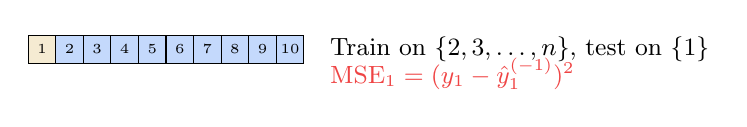
\begin{tikzpicture}[scale=0.7]
  \foreach \j in {1,...,10} {
    \ifnum\j=1
      \fill[beige] ({(\j-1)*0.5}, 0) rectangle ({(\j)*0.5}, 0.5);
    \else
      \fill[accent!30] ({(\j-1)*0.5}, 0) rectangle ({(\j)*0.5}, 0.5);
    \fi
    \draw ({(\j-1)*0.5}, 0) rectangle ({(\j)*0.5}, 0.5);
    \node[font=\tiny] at ({(\j-0.5)*0.5}, 0.25) {\j};
  }
  \node[right, font=\small] at (5.3, 0.25) {Train on $\{2,3,\ldots,n\}$, test on $\{1\}$};
  \node[right, font=\small, softred] at (5.3, -0.2) {$\text{MSE}_1 = (y_1 - \hat{y}_1^{(-1)})^2$};
\end{tikzpicture}
\end{center}

\textbf{Iteration $i = 2$:}

\begin{center}
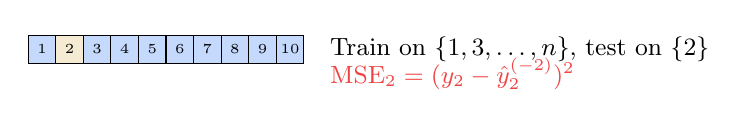
\begin{tikzpicture}[scale=0.7]
  \foreach \j in {1,...,10} {
    \ifnum\j=2
      \fill[beige] ({(\j-1)*0.5}, 0) rectangle ({(\j)*0.5}, 0.5);
    \else
      \fill[accent!30] ({(\j-1)*0.5}, 0) rectangle ({(\j)*0.5}, 0.5);
    \fi
    \draw ({(\j-1)*0.5}, 0) rectangle ({(\j)*0.5}, 0.5);
    \node[font=\tiny] at ({(\j-0.5)*0.5}, 0.25) {\j};
  }
  \node[right, font=\small] at (5.3, 0.25) {Train on $\{1,3,\ldots,n\}$, test on $\{2\}$};
  \node[right, font=\small, softred] at (5.3, -0.2) {$\text{MSE}_2 = (y_2 - \hat{y}_2^{(-2)})^2$};
\end{tikzpicture}
\end{center}

\vspace{0.3em}
$\vdots$ \quad (repeat for all $n$ observations)

$$\text{CV}_{(n)} = \frac{1}{n}(\text{MSE}_1 + \text{MSE}_2 + \cdots + \text{MSE}_n)$$

Every observation gets a turn as the test point!
\end{frame}


\begin{frame}{LOOCV: Numerical Computation (Mini Example)}

\textbf{Toy data:} $n = 5$, simple linear regression $Y = \beta_0 + \beta_1 X$

\begin{columns}
\column{0.4\textwidth}
\begin{tabular}{cc}
\toprule
$x_i$ & $y_i$ \\
\midrule
1 & 2.1 \\
2 & 3.9 \\
3 & 5.0 \\
4 & 6.8 \\
5 & 8.2 \\
\bottomrule
\end{tabular}

\column{0.55\textwidth}
\textbf{Leave out obs 3:}

Train on $\{(1,2.1),(2,3.9),(4,6.8),(5,8.2)\}$

Fit: $\hat{Y} = 0.43 + 1.54X$

Predict: $\hat{y}_3 = 0.43 + 1.54(3) = 5.05$

$\text{MSE}_3 = (5.0 - 5.05)^2 = 0.0025$
\end{columns}

\vspace{0.5em}
\textbf{All iterations:}

\begin{center}
\begin{tabular}{ccccc}
\toprule
Leave out & $\hat{y}_i^{(-i)}$ & $e_i$ & $e_i^2$ \\
\midrule
1 & 1.88 & 0.22 & 0.048 \\
2 & 3.88 & 0.02 & 0.000 \\
3 & 5.05 & $-0.05$ & 0.003 \\
4 & 6.72 & 0.08 & 0.006 \\
5 & 8.22 & $-0.02$ & 0.000 \\
\bottomrule
\end{tabular}
\end{center}

$\text{CV}_{(5)} = (0.048 + 0.000 + 0.003 + 0.006 + 0.000)/5 = 0.011$
\end{frame}


\begin{frame}{The Shortcut Formula: Leverage-Adjusted Residuals}

\textbf{Regular LOOCV:} Refit model $n$ times $\Rightarrow$ expensive

\textbf{Shortcut:} Fit model \textbf{once}, adjust residuals by leverage

$$\text{CV}_{(n)} = \frac{1}{n}\sum_{i=1}^{n}\left(\frac{y_i - \hat{y}_i}{1 - h_i}\right)^2 = \frac{1}{n}\sum_{i=1}^{n}\left(\frac{e_i}{1 - h_i}\right)^2$$

\begin{columns}
\column{0.5\textwidth}
\textbf{Why does this work?}

High-leverage point: $h_i$ close to 1

$\Rightarrow$ Point strongly influences its own fit

$\Rightarrow$ Residual $e_i$ is artificially small

$\Rightarrow$ Dividing by $(1-h_i)$ inflates it back

\column{0.45\textwidth}
\textbf{Numerical verification:}

\begin{tabular}{cccc}
\toprule
$i$ & $e_i$ & $h_i$ & $\frac{e_i}{1-h_i}$ \\
\midrule
1 & 0.18 & 0.40 & 0.30 \\
2 & 0.02 & 0.20 & 0.03 \\
3 & $-0.04$ & 0.13 & $-0.05$ \\
4 & 0.06 & 0.20 & 0.08 \\
5 & $-0.01$ & 0.40 & $-0.02$ \\
\bottomrule
\end{tabular}

\footnotesize Edge obs (1,5): largest $h_i$, largest correction
\end{columns}
\end{frame}


\begin{frame}{$k$-Fold CV: Worked Example with $k=5$}

\textbf{Auto data:} $n = 392$, quadratic model, $k = 5$

Each fold has $\approx 78$ observations

\vspace{0.3em}
\begin{center}
\begin{tabular}{ccccc}
\toprule
Fold & Train $n$ & Test $n$ & MSE$_i$ \\
\midrule
1 & 314 & 78 & 18.95 \\
2 & 314 & 78 & 19.82 \\
3 & 314 & 78 & 19.41 \\
4 & 314 & 78 & 18.73 \\
5 & 314 & 78 & 19.34 \\
\bottomrule
\end{tabular}
\end{center}

$$\text{CV}_{(5)} = \frac{18.95 + 19.82 + 19.41 + 18.73 + 19.34}{5} = 19.25$$

\textit{Very close to the LOOCV estimate of 19.25 --- but 78$\times$ faster!}
\end{frame}


\begin{frame}{Stratified $k$-Fold CV: For Classification}
\begin{columns}
\column{0.55\textwidth}
\textbf{Problem:} With imbalanced classes, a random fold might get \textbf{zero} positive examples!

\vspace{0.3em}
\textbf{Default data:} 3.3\% default rate

In 10-fold: each fold has $\sim 1000$ obs

Expected defaults per fold: $\sim 33$

\vspace{0.3em}
\textbf{Stratified CV:}

Each fold has the \textbf{same proportion} of each class as the full dataset

$\Rightarrow$ More stable error estimates

\column{0.4\textwidth}
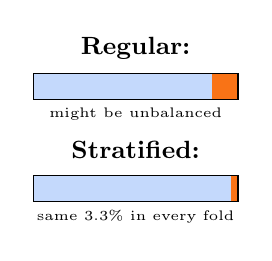
\begin{tikzpicture}[scale=0.65]
  % Regular fold (unbalanced)
  \node[font=\small\bfseries] at (2, 4) {Regular:};
  \fill[accent!30] (0, 3) rectangle (3.5, 3.5);
  \fill[orange] (3.5, 3) rectangle (4, 3.5);
  \draw (0,3) rectangle (4, 3.5);
  \node[font=\tiny] at (2, 2.7) {might be unbalanced};

  % Stratified fold
  \node[font=\small\bfseries] at (2, 2) {Stratified:};
  \fill[accent!30] (0, 1) rectangle (3.87, 1.5);
  \fill[orange] (3.87, 1) rectangle (4, 1.5);
  \draw (0,1) rectangle (4, 1.5);
  \node[font=\tiny] at (2, 0.7) {same 3.3\% in every fold};
\end{tikzpicture}

\vspace{0.3em}
\footnotesize R: \texttt{caret::createFolds(y, k=10)}\\
automatically stratifies
\end{columns}
\end{frame}


\begin{frame}{CV for Model Selection: Polynomial Degree}
\begin{columns}
\column{0.5\textwidth}
\textbf{Goal:} Choose $d$ in

$\text{mpg} \sim \text{poly(hp}, d)$

\vspace{0.3em}
\begin{tabular}{ccc}
\toprule
$d$ & LOOCV & 10-fold \\
\midrule
1 & 24.23 & 24.27 \\
\textcolor{softgreen}{2} & \textcolor{softgreen}{19.25} & \textcolor{softgreen}{19.27} \\
3 & 19.33 & 19.35 \\
4 & 19.42 & 19.29 \\
5 & 19.03 & 19.03 \\
7 & 18.83 & 19.12 \\
10 & 19.49 & 20.96 \\
\bottomrule
\end{tabular}

\column{0.45\textwidth}
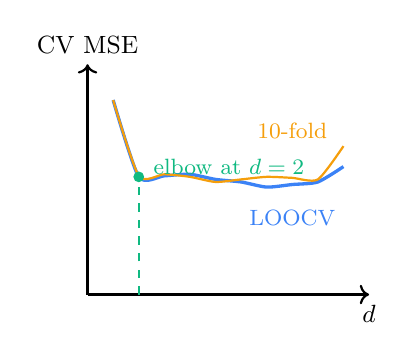
\begin{tikzpicture}[scale=0.65]
  \draw[->, thick] (0,0) -- (5.5,0) node[below] {\small $d$};
  \draw[->, thick] (0,0) -- (0,4.5) node[above] {\small CV MSE};
  % LOOCV
  \draw[accent, very thick, smooth, tension=0.4] plot coordinates {(0.5,3.8)(1,2.3)(1.5,2.32)(2,2.35)(2.5,2.25)(3,2.2)(3.5,2.1)(4,2.15)(4.5,2.2)(5,2.5)};
  % 10-fold
  \draw[amber, thick, smooth, tension=0.4] plot coordinates {(0.5,3.8)(1,2.32)(1.5,2.35)(2,2.3)(2.5,2.2)(3,2.25)(3.5,2.3)(4,2.28)(4.5,2.25)(5,2.9)};
  % Elbow
  \draw[softgreen, thick, dashed] (1, 0) -- (1, 2.3);
  \fill[softgreen] (1, 2.3) circle (3pt);
  \node[softgreen, right, font=\footnotesize] at (1.1, 2.5) {elbow at $d=2$};
  \node[accent, font=\footnotesize] at (4, 1.5) {LOOCV};
  \node[amber, font=\footnotesize] at (4, 3.2) {10-fold};
\end{tikzpicture}

\textbf{Both methods agree:}

$d = 2$ is the sweet spot

Higher degrees add complexity\\
without reducing error
\end{columns}
\end{frame}


\begin{frame}{CV for Model Selection: Comparing Entire Models}

\textbf{Which model predicts mpg best?}

\vspace{0.3em}
\begin{center}
\begin{tabular}{lcc}
\toprule
Model & 10-fold CV MSE & \# predictors \\
\midrule
mpg $\sim$ horsepower & 24.27 & 1 \\
mpg $\sim$ poly(hp, 2) & 19.27 & 2 \\
mpg $\sim$ weight & 18.95 & 1 \\
mpg $\sim$ weight + year & 14.82 & 2 \\
\textcolor{softgreen}{mpg $\sim$ weight + year + origin} & \textcolor{softgreen}{12.55} & \textcolor{softgreen}{3} \\
mpg $\sim$ . $-$ name & 11.58 & 7 \\
\bottomrule
\end{tabular}
\end{center}

\vspace{0.3em}
\begin{itemize}
  \item Weight alone beats poly(hp, 2)!
  \item Adding year provides a large improvement
  \item Full model is best but uses 7 predictors
  \item \textbf{Weight + year + origin}: good trade-off
\end{itemize}
\end{frame}


\begin{frame}{CV for Classification: Default Dataset}
\begin{columns}
\column{0.5\textwidth}
\textbf{Logistic regression:}

$\text{default} \sim \text{balance}$

\vspace{0.3em}
10-fold CV error rate:

\begin{tabular}{cc}
\toprule
Fold & Error rate \\
\midrule
1 & 2.3\% \\
2 & 2.8\% \\
3 & 2.5\% \\
$\vdots$ & $\vdots$ \\
10 & 2.7\% \\
\midrule
\textbf{Average} & \textbf{2.6\%} \\
\bottomrule
\end{tabular}

\column{0.45\textwidth}
\textbf{But what about sensitivity?}

\vspace{0.3em}
10-fold CV can also report:
\begin{itemize}
  \item Average sensitivity per fold
  \item Average AUC per fold
  \item Average F1 per fold
\end{itemize}

\vspace{0.3em}
\textbf{Accuracy alone is misleading!}

(Recall: predicting ``No'' always gives 96.7\% accuracy)

\vspace{0.3em}
\footnotesize R: Use \texttt{caret::train()} for classification metrics per fold
\end{columns}
\end{frame}


\begin{frame}{The ``One Standard Error Rule''}
\begin{columns}
\column{0.55\textwidth}
\textbf{Problem:}

The model with the \textit{lowest} CV error may be too complex

\vspace{0.3em}
\textbf{One-SE Rule:}

Choose the \textbf{simplest model} whose CV error is within one standard error of the minimum

\vspace{0.5em}
\textbf{Why?}

\begin{itemize}
  \item Simpler models are more interpretable
  \item The ``best'' model might be winning by noise
  \item Conservative: prefer parsimony
\end{itemize}

\vspace{0.3em}
\textit{Used heavily in Lasso/Ridge (Week 4)}

\column{0.4\textwidth}
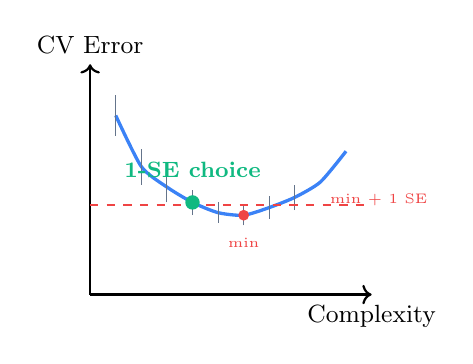
\begin{tikzpicture}[scale=0.65]
  \draw[->, thick] (0,0) -- (5.5,0) node[below] {\small Complexity};
  \draw[->, thick] (0,0) -- (0,4.5) node[above] {\small CV Error};
  % CV curve
  \draw[accent, very thick, smooth, tension=0.4] plot coordinates {(0.5,3.5)(1,2.5)(1.5,2.1)(2,1.8)(2.5,1.6)(3,1.55)(3.5,1.7)(4,1.9)(4.5,2.2)(5,2.8)};
  % Error bars
  \foreach \x/\y/\se in {0.5/3.5/0.4, 1/2.5/0.35, 1.5/2.1/0.3, 2/1.8/0.25, 2.5/1.6/0.2, 3/1.55/0.2, 3.5/1.7/0.22, 4/1.9/0.25} {
    \draw[muted] (\x, \y-\se) -- (\x, \y+\se);
  }
  % Min
  \fill[softred] (3, 1.55) circle (3pt);
  \node[softred, below] at (3, 1.3) {\tiny min};
  % 1 SE line
  \draw[softred, dashed] (0, 1.75) -- (5.5, 1.75);
  \node[softred, right, font=\tiny] at (4.5, 1.85) {min + 1 SE};
  % 1 SE choice
  \fill[softgreen] (2, 1.8) circle (4pt);
  \node[softgreen, above, font=\footnotesize] at (2, 2.1) {\textbf{1-SE choice}};
\end{tikzpicture}
\end{columns}
\end{frame}


\begin{frame}{Repeated $k$-Fold CV}
\begin{columns}
\column{0.55\textwidth}
\textbf{Problem:} Even 10-fold CV has some randomness (from the random split into folds)

\vspace{0.3em}
\textbf{Solution:} Repeat the entire $k$-fold procedure $R$ times

\begin{enumerate}
  \item Run 10-fold CV with seed 1 $\Rightarrow$ CV$_1$
  \item Run 10-fold CV with seed 2 $\Rightarrow$ CV$_2$
  \item[] $\vdots$
  \item[$R$.] Run 10-fold CV with seed $R$ $\Rightarrow$ CV$_R$
\end{enumerate}

Final estimate: $\frac{1}{R}\sum_{r=1}^{R} \text{CV}_r$

\column{0.4\textwidth}
\textbf{How many repeats?}

\begin{tabular}{cc}
\toprule
$R$ & SE reduction \\
\midrule
1 & baseline \\
5 & $\div \sqrt{5} \approx 2.2\times$ \\
10 & $\div \sqrt{10} \approx 3.2\times$ \\
\bottomrule
\end{tabular}

\vspace{0.5em}
Typical: $R = 5$ or $R = 10$

\vspace{0.3em}
\footnotesize R: \texttt{caret::trainControl(}\\
\texttt{\quad method="repeatedcv",}\\
\texttt{\quad number=10, repeats=5)}
\end{columns}
\end{frame}


\begin{frame}{Nested CV: The Gold Standard}
\begin{columns}
\column{0.55\textwidth}
\textbf{Problem:}

If we use CV to \textbf{select} a model AND \textbf{estimate} its error, the estimate is biased (optimistic)

\vspace{0.3em}
\textbf{Solution: Nested CV}

\begin{itemize}
  \item \textbf{Outer loop:} 10-fold CV estimates test error
  \item \textbf{Inner loop:} 5-fold CV selects the model
\end{itemize}

\vspace{0.3em}
The inner loop tunes, the outer loop evaluates

\column{0.4\textwidth}
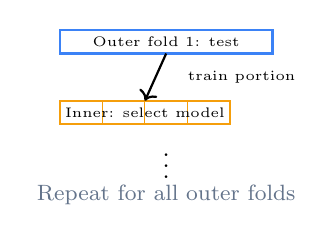
\begin{tikzpicture}[scale=0.6]
  % Outer folds
  \draw[accent, thick] (0, 3.5) rectangle (4.5, 4);
  \node[font=\tiny] at (2.25, 3.75) {Outer fold 1: test};
  % Inner folds
  \draw[amber, thick] (0, 2) rectangle (3.6, 2.5);
  \draw[amber] (0.9, 2) -- (0.9, 2.5);
  \draw[amber] (1.8, 2) -- (1.8, 2.5);
  \draw[amber] (2.7, 2) -- (2.7, 2.5);
  \node[font=\tiny] at (1.8, 2.25) {Inner: select model};
  \draw[->, thick] (2.25, 3.5) -- (1.8, 2.5);
  \node[font=\tiny, right] at (2.5, 3) {train portion};
  % Repeat
  \node[font=\small] at (2.25, 1.3) {$\vdots$};
  \node[font=\footnotesize, muted] at (2.25, 0.5) {Repeat for all outer folds};
\end{tikzpicture}

\vspace{0.3em}
\footnotesize Computationally expensive\\but unbiased
\end{columns}
\end{frame}


\begin{frame}{Bootstrap: The Key Insight}

\textbf{Why does resampling with replacement mimic new datasets?}

\begin{columns}
\column{0.55\textwidth}
\textbf{The plug-in principle:}

We don't know the population distribution $F$

But our sample $\hat{F}$ is our best estimate of $F$

Drawing from $\hat{F}$ with replacement $\approx$ drawing from $F$

\vspace{0.5em}
\textbf{As $n \to \infty$:}

$\hat{F} \to F$, so bootstrap $\to$ exact

\vspace{0.3em}
For finite $n$: approximate, but usually very good

\column{0.4\textwidth}
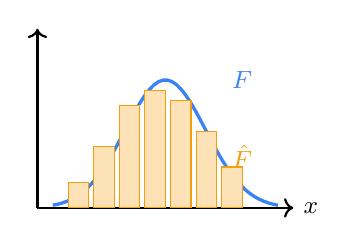
\begin{tikzpicture}[scale=0.65]
  \draw[->, thick] (0,0) -- (5,0) node[right] {\small $x$};
  \draw[->, thick] (0,0) -- (0,3.5);
  % True distribution
  \draw[accent, very thick, domain=0.3:4.7, samples=50] plot (\x, {2.5*exp(-0.8*(\x-2.5)*(\x-2.5))});
  \node[accent] at (4, 2.5) {\small $F$};
  % Empirical distribution (histogram)
  \foreach \x/\h in {0.8/0.5, 1.3/1.2, 1.8/2.0, 2.3/2.3, 2.8/2.1, 3.3/1.5, 3.8/0.8} {
    \fill[amber!30] (\x-0.2, 0) rectangle (\x+0.2, \h);
    \draw[amber] (\x-0.2, 0) rectangle (\x+0.2, \h);
  }
  \node[amber] at (4, 1.0) {\small $\hat{F}$};
\end{tikzpicture}

\vspace{0.2em}
\footnotesize The histogram approximates\\the true density
\end{columns}
\end{frame}


\begin{frame}{Bootstrap: Which Observations Get Selected?}

\textbf{Each bootstrap sample:} draw $n$ times with replacement

\begin{columns}
\column{0.5\textwidth}
\textbf{Original:} $\{1, 2, 3, 4, 5, 6, 7, 8\}$

\textbf{Sample 1:} $\{2, 5, 5, 1, 7, 3, 5, 8\}$

$\Rightarrow$ Obs 5 appears 3 times!\\
$\Rightarrow$ Obs 4, 6 are missing

\vspace{0.3em}
\textbf{Sample 2:} $\{3, 1, 1, 6, 4, 3, 8, 2\}$

$\Rightarrow$ Obs 1, 3 appear twice\\
$\Rightarrow$ Obs 5, 7 are missing

\column{0.45\textwidth}
\textbf{Probability of inclusion:}

$P(\text{obs } j \text{ included}) = 1 - \left(1 - \frac{1}{n}\right)^n$

\vspace{0.3em}
\begin{tabular}{cc}
\toprule
$n$ & $P(\text{included})$ \\
\midrule
5 & 67.2\% \\
10 & 65.1\% \\
100 & 63.4\% \\
$\infty$ & $1 - e^{-1} = 63.2\%$ \\
\bottomrule
\end{tabular}

\vspace{0.3em}
$\approx 36.8\%$ are \textbf{out-of-bag (OOB)}
\end{columns}
\end{frame}


\begin{frame}{Bootstrap SE: Step-by-Step Example}

\textbf{Estimate the SE of the sample mean} $\bar{X}$

\begin{columns}
\column{0.45\textwidth}
\textbf{Original data:} $\{3, 7, 2, 5, 8\}$

$\bar{X} = 5.0$

\vspace{0.3em}
$B = 4$ bootstrap samples:

\begin{tabular}{cc}
\toprule
Sample & $\bar{X}^{*b}$ \\
\midrule
$\{7,3,3,5,7\}$ & 5.0 \\
$\{8,2,7,2,5\}$ & 4.8 \\
$\{5,5,8,3,2\}$ & 4.6 \\
$\{3,8,7,7,5\}$ & 6.0 \\
\bottomrule
\end{tabular}

\column{0.5\textwidth}
$\bar{\hat{X}}^* = (5.0 + 4.8 + 4.6 + 6.0)/4 = 5.1$

\vspace{0.3em}
$\text{SE}_B = \sqrt{\frac{1}{3}\sum_{b=1}^{4}(\bar{X}^{*b} - 5.1)^2}$

\vspace{0.3em}
$= \sqrt{\frac{(0.01 + 0.09 + 0.25 + 0.81)}{3}}$

$= \sqrt{0.387} = 0.622$

\vspace{0.3em}
\textbf{Formula SE:} $s/\sqrt{n} = 2.55/\sqrt{5} = 1.14$

\vspace{0.3em}
\footnotesize (With only $B=4$, bootstrap is noisy. Use $B \geq 1000$!)
\end{columns}
\end{frame}


\begin{frame}{How Many Bootstrap Samples $B$?}
\begin{columns}
\column{0.5\textwidth}
\textbf{Rule of thumb:}

\begin{tabular}{ll}
\toprule
Goal & $B$ \\
\midrule
Standard errors & $B \geq 1{,}000$ \\
Confidence intervals & $B \geq 5{,}000$ \\
Hypothesis testing & $B \geq 10{,}000$ \\
\bottomrule
\end{tabular}

\vspace{0.5em}
More $B$ = more precise SE estimate

But diminishing returns past $B \approx 10{,}000$

\column{0.45\textwidth}
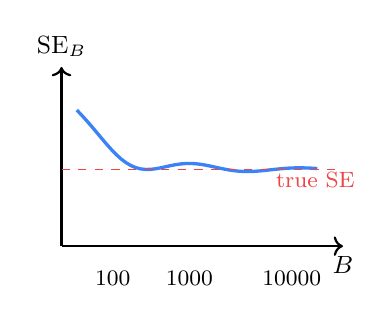
\begin{tikzpicture}[scale=0.65]
  \draw[->, thick] (0,0) -- (5.5,0) node[below] {\small $B$};
  \draw[->, thick] (0,0) -- (0,3.5) node[above] {\small $\text{SE}_B$};
  \draw[accent, very thick, domain=0.3:5, samples=50] plot (\x, {1.5 + 1.5*exp(-1.5*\x) + 0.3*sin(\x*3 r)*exp(-0.5*\x)});
  \draw[softred, dashed] (0, 1.5) -- (5.5, 1.5);
  \node[softred, right, font=\footnotesize] at (4, 1.3) {true SE};
  \node[below, font=\footnotesize] at (1, -0.3) {100};
  \node[below, font=\footnotesize] at (2.5, -0.3) {1000};
  \node[below, font=\footnotesize] at (4.5, -0.3) {10000};
\end{tikzpicture}

\vspace{0.2em}
\footnotesize Stabilizes around $B = 1000$
\end{columns}
\end{frame}


\begin{frame}{Bootstrap vs.\ Formula: When They Disagree}
\begin{columns}
\column{0.5\textwidth}
\textbf{Auto data: SLR} (mpg $\sim$ hp)

\begin{tabular}{lcc}
\toprule
 & Formula & Bootstrap \\
\midrule
$\text{SE}(\hat{\beta}_0)$ & 0.717 & \textcolor{softred}{0.860} \\
$\text{SE}(\hat{\beta}_1)$ & 0.006 & \textcolor{softred}{0.007} \\
\bottomrule
\end{tabular}

Bootstrap SEs are \textbf{larger}!

\vspace{0.3em}
\textbf{Why?}

Formula assumes $Y = \beta_0 + \beta_1 X + \varepsilon$

But true relationship is non-linear

$\Rightarrow$ Formula SEs are too optimistic

\column{0.45\textwidth}
\textbf{Auto data: Quadratic} (mpg $\sim$ hp + hp$^2$)

\begin{tabular}{lcc}
\toprule
 & Formula & Bootstrap \\
\midrule
$\text{SE}(\hat{\beta}_0)$ & 1.800 & 1.870 \\
$\text{SE}(\hat{\beta}_1)$ & 0.031 & 0.030 \\
$\text{SE}(\hat{\beta}_2)$ & 0.0001 & 0.0001 \\
\bottomrule
\end{tabular}

Now they \textbf{agree}!

\vspace{0.3em}
\textcolor{softgreen}{Quadratic model is correct}\\
$\Rightarrow$ formula assumptions hold\\
$\Rightarrow$ both methods give same answer
\end{columns}
\end{frame}


\begin{frame}{Bootstrap for Prediction Intervals}
\begin{columns}
\column{0.55\textwidth}
\textbf{Beyond standard errors:}

Bootstrap can estimate \textbf{any} quantity's distribution

\vspace{0.3em}
\textbf{Prediction at $x_0 = 100$ hp:}

\begin{enumerate}
  \item For each bootstrap sample $b$:
  \begin{enumerate}
    \item[a.] Fit model on sample $b$
    \item[b.] Predict $\hat{y}_0^{*b}$ at $x_0 = 100$
    \item[c.] Add noise: $y_0^{*b} = \hat{y}_0^{*b} + \varepsilon^{*b}$
  \end{enumerate}
  \item Use percentiles of $\{y_0^{*1}, \ldots, y_0^{*B}\}$\\as prediction interval
\end{enumerate}

\column{0.4\textwidth}
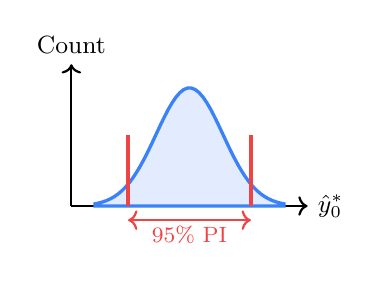
\begin{tikzpicture}[scale=0.6]
  \draw[->, thick] (0,0) -- (5,0) node[right] {\small $\hat{y}_0^*$};
  \draw[->, thick] (0,0) -- (0,3) node[above] {\small Count};
  % Bootstrap distribution of predictions
  \draw[accent, very thick, domain=0.5:4.5, samples=50, fill=accent!15] plot (\x, {2.5*exp(-1*(\x-2.5)*(\x-2.5))}) -- (4.5,0) -- (0.5,0) -- cycle;
  % CI
  \draw[softred, very thick] (1.2, 0) -- (1.2, 1.5);
  \draw[softred, very thick] (3.8, 0) -- (3.8, 1.5);
  \draw[<->, softred, thick] (1.2, -0.3) -- (3.8, -0.3);
  \node[softred, font=\footnotesize] at (2.5, -0.6) {95\% PI};
\end{tikzpicture}

\vspace{0.3em}
\footnotesize Much wider than the\\confidence interval!
\end{columns}
\end{frame}


\begin{frame}{Out-of-Bag Error: Bootstrap Meets CV}

\textbf{Key observation:} Each bootstrap sample leaves out $\sim 36.8\%$ of observations

\begin{columns}
\column{0.55\textwidth}
\textbf{OOB error estimation:}

\begin{enumerate}
  \item For bootstrap sample $b$, predict the $\sim 36.8\%$ left-out observations
  \item Average these predictions across all bootstrap samples
  \item This gives an estimate of test error!
\end{enumerate}

\vspace{0.3em}
\textbf{Advantage:}

No separate validation set needed --- it's ``free'' from the bootstrap

\column{0.4\textwidth}
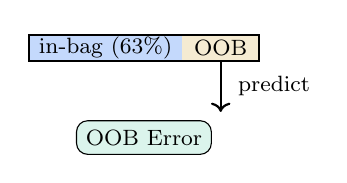
\begin{tikzpicture}[scale=0.65]
  % Bootstrap sample
  \fill[accent!30] (0, 2.5) rectangle (3, 3);
  \fill[beige] (3, 2.5) rectangle (4.5, 3);
  \draw[thick] (0, 2.5) rectangle (4.5, 3);
  \node[font=\footnotesize] at (1.5, 2.75) {in-bag (63\%)};
  \node[font=\footnotesize] at (3.75, 2.75) {OOB};

  % Arrow
  \draw[->, thick] (3.75, 2.5) -- (3.75, 1.5);
  \node[font=\footnotesize, right] at (3.9, 2) {predict};

  % OOB predictions
  \node[draw, fill=softgreen!15, rounded corners, font=\footnotesize] at (2.25, 1) {OOB Error};
\end{tikzpicture}

\vspace{0.3em}
\textit{Used in Random Forests (Week 6) as the default error estimate!}
\end{columns}
\end{frame}


\begin{frame}{CV for Tuning Hyperparameters: KNN Example}

\textbf{Question:} What is the best $K$ for KNN on the Default data?

\vspace{0.3em}
\begin{columns}
\column{0.45\textwidth}
\textbf{10-fold CV results:}

\begin{tabular}{cc}
\toprule
$K$ & CV Error Rate \\
\midrule
1 & 3.8\% \\
3 & 3.2\% \\
5 & 2.9\% \\
10 & 2.7\% \\
20 & 2.6\% \\
\textcolor{softgreen}{50} & \textcolor{softgreen}{2.5\%} \\
100 & 2.6\% \\
\bottomrule
\end{tabular}

\column{0.5\textwidth}
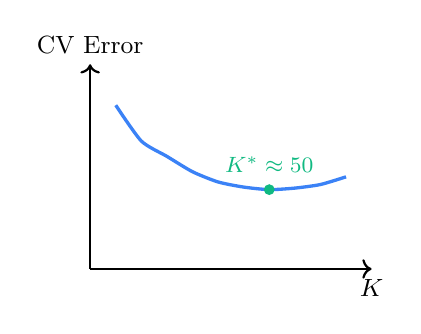
\begin{tikzpicture}[scale=0.65]
  \draw[->, thick] (0,0) -- (5.5,0) node[below] {\small $K$};
  \draw[->, thick] (0,0) -- (0,4) node[above] {\small CV Error};
  % CV curve
  \draw[accent, very thick, smooth, tension=0.4] plot coordinates {(0.5,3.2)(1,2.5)(1.5,2.2)(2,1.9)(2.5,1.7)(3,1.6)(3.5,1.55)(4,1.58)(4.5,1.65)(5,1.8)};
  \fill[softgreen] (3.5, 1.55) circle (3pt);
  \node[softgreen, above, font=\footnotesize] at (3.5, 1.7) {$K^* \approx 50$};
\end{tikzpicture}

\vspace{0.3em}
\textbf{Workflow:}

\begin{enumerate}
  \item CV for each $K$
  \item Pick $K^*$ with lowest CV error
  \item Refit KNN with $K^*$ on all data
\end{enumerate}
\end{columns}
\end{frame}


\begin{frame}{Data Leakage: The Silent Killer}

\begin{columns}
\column{0.48\textwidth}
\textbf{\textcolor{softred}{Wrong:}}

\begin{enumerate}
  \item Standardize ALL data
  \item Then split into folds
  \item Run CV
\end{enumerate}

\vspace{0.2em}
The test fold ``knows'' the mean and SD of the training data

$\Rightarrow$ CV error is \textbf{optimistic}

$\Rightarrow$ Real test error is \textbf{worse}

\column{0.48\textwidth}
\textbf{\textcolor{softgreen}{Right:}}

\begin{enumerate}
  \item Split into folds
  \item For each fold:
  \begin{enumerate}
    \item[a.] Compute mean/SD on \textbf{train only}
    \item[b.] Standardize train with those stats
    \item[c.] Apply \textbf{same} stats to test fold
  \end{enumerate}
\end{enumerate}

\vspace{0.2em}
Test fold is truly unseen!
\end{columns}

\vspace{0.5em}
\centering
\fbox{\parbox{0.7\textwidth}{\centering
\textbf{Rule:} Any computation on data must happen \textbf{inside} each CV fold,\\
not before splitting!}}
\end{frame}


\begin{frame}{Bootstrap Confidence Intervals: Three Methods}

\begin{center}
\begin{tabular}{llc}
\toprule
Method & Formula & Assumes Normal? \\
\midrule
Normal & $\hat{\theta} \pm z_{\alpha/2} \cdot \text{SE}_B$ & Yes \\
Percentile & $[\hat{\theta}^*_{\alpha/2}, \;\; \hat{\theta}^*_{1-\alpha/2}]$ & No \\
BCa (bias-corrected) & Adjusted percentiles & No \\
\bottomrule
\end{tabular}
\end{center}

\vspace{0.5em}
\begin{columns}
\column{0.5\textwidth}
\textbf{Portfolio example ($\hat{\alpha} = 0.576$):}

\begin{tabular}{lc}
\toprule
Method & 95\% CI \\
\midrule
Normal & $[0.40, \; 0.75]$ \\
Percentile & $[0.39, \; 0.74]$ \\
BCa & $[0.41, \; 0.76]$ \\
\bottomrule
\end{tabular}

All three are similar here

\column{0.45\textwidth}
\textbf{When they differ:}

If $\hat{\theta}^*$ distribution is \textbf{skewed}, percentile and BCa are better

\vspace{0.3em}
\footnotesize R: \texttt{boot.ci(boot.out,}\\
\texttt{\quad type=c("norm","perc","bca"))}
\end{columns}
\end{frame}


\begin{frame}{Parametric vs.\ Non-Parametric Bootstrap}
\begin{columns}
\column{0.48\textwidth}
\textbf{Non-parametric} (standard):

Resample $(x_i, y_i)$ pairs with replacement

No model assumptions

\vspace{0.3em}
\textbf{What we've been doing!}

\vspace{0.5em}
\textbf{Use when:}
\begin{itemize}
  \item Model may be wrong
  \item Want robust SEs
  \item General-purpose
\end{itemize}

\column{0.48\textwidth}
\textbf{Parametric:}

\begin{enumerate}
  \item Fit model: $\hat{Y} = \hat{\beta}_0 + \hat{\beta}_1 X$
  \item Generate new $Y^* = \hat{Y} + \varepsilon^*$\\where $\varepsilon^* \sim N(0, \hat{\sigma}^2)$
  \item Refit on $(X, Y^*)$
\end{enumerate}

\vspace{0.3em}
\textbf{Use when:}
\begin{itemize}
  \item Model is trusted
  \item Want more efficiency
  \item Especially with small $n$
\end{itemize}
\end{columns}
\end{frame}


\begin{frame}{What Can Go Wrong with the Bootstrap?}

\begin{enumerate}
  \item \textbf{Small sample size}
  \begin{itemize}
    \item[$\circ$] $n < 20$: bootstrap distribution may be poor
    \item[$\circ$] Not enough ``diversity'' in resamples
  \end{itemize}

  \vspace{0.3em}
  \item \textbf{Dependent data}
  \begin{itemize}
    \item[$\circ$] Time series: observations are correlated
    \item[$\circ$] Standard bootstrap breaks independence assumption
    \item[$\circ$] Use \textbf{block bootstrap} instead
  \end{itemize}

  \vspace{0.3em}
  \item \textbf{Extreme values / heavy tails}
  \begin{itemize}
    \item[$\circ$] Bootstrap may miss rare events
    \item[$\circ$] Large outliers dominate some resamples
  \end{itemize}

  \vspace{0.3em}
  \item \textbf{Not enough $B$}
  \begin{itemize}
    \item[$\circ$] $B = 50$ is not enough! Use $B \geq 1000$
  \end{itemize}
\end{enumerate}
\end{frame}


\begin{frame}{Computational Cost Comparison}

\begin{center}
\begin{tabular}{lccc}
\toprule
Method & Model fits & Auto ($n=392$) & Default ($n=10$k) \\
\midrule
Validation set & 1 & instant & instant \\
5-fold CV & 5 & instant & fast \\
10-fold CV & 10 & instant & fast \\
LOOCV & $n$ & 392 fits & 10,000 fits \\
LOOCV (shortcut) & 1 & instant & instant \\
Bootstrap ($B$=1000) & 1,000 & fast & moderate \\
\bottomrule
\end{tabular}
\end{center}

\vspace{0.5em}
\textbf{Key points:}
\begin{itemize}
  \item The LOOCV shortcut only works for \textbf{linear} models
  \item For complex models (trees, neural nets): LOOCV is prohibitive
  \item 10-fold CV: always practical --- the default choice
\end{itemize}
\end{frame}


\begin{frame}{When to Use Which Method: Decision Guide}

\begin{center}
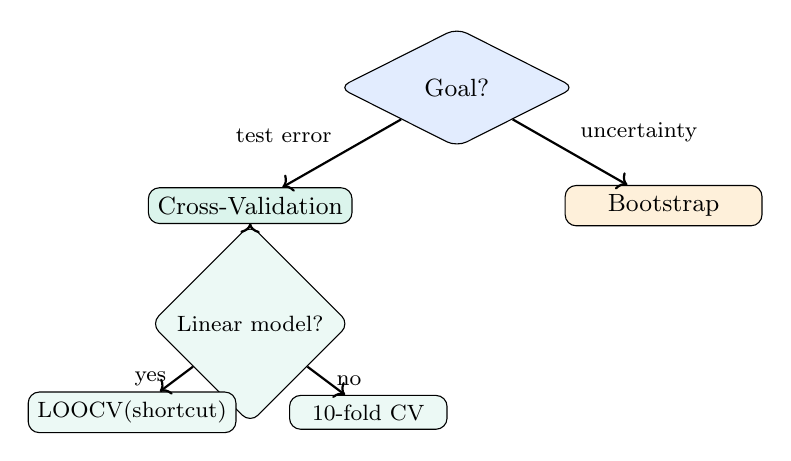
\begin{tikzpicture}[scale=0.75, every node/.style={font=\small}]
  \node[draw, fill=accent!15, rounded corners, diamond, minimum width=3cm, minimum height=1.5cm] (q1) at (0,4) {Goal?};

  \node[draw, fill=softgreen!15, rounded corners, minimum width=2.5cm] (cv) at (-3.5,2) {Cross-Validation};
  \node[draw, fill=amber!15, rounded corners, minimum width=2.5cm] (bs) at (3.5,2) {Bootstrap};

  \node[draw, fill=softgreen!8, rounded corners, diamond, minimum width=2.5cm, minimum height=1cm, font=\footnotesize] (q2) at (-3.5,0) {Linear model?};

  \node[draw, fill=softgreen!8, rounded corners, font=\footnotesize, minimum width=2cm] (loo) at (-5.5,-1.5) {LOOCV\\(shortcut)};
  \node[draw, fill=softgreen!8, rounded corners, font=\footnotesize, minimum width=2cm] (kf) at (-1.5,-1.5) {10-fold CV};

  \draw[->, thick] (q1) -- (cv) node[midway, above left, font=\footnotesize] {test error};
  \draw[->, thick] (q1) -- (bs) node[midway, above right, font=\footnotesize] {uncertainty};
  \draw[->, thick] (cv) -- (q2);
  \draw[->, thick] (q2) -- (loo) node[midway, left, font=\footnotesize] {yes};
  \draw[->, thick] (q2) -- (kf) node[midway, right, font=\footnotesize] {no};
\end{tikzpicture}
\end{center}
\end{frame}


\begin{frame}{Real-World Example: Choosing a Spam Filter}

\textbf{Scenario:} Compare 4 classifiers for spam detection

\vspace{0.3em}
\begin{center}
\begin{tabular}{lccc}
\toprule
Model & 10-fold CV Error & CV Sensitivity & CV AUC \\
\midrule
Logistic & 7.2\% & 82\% & 0.94 \\
LDA & 8.1\% & 78\% & 0.91 \\
\textcolor{softgreen}{QDA} & \textcolor{softgreen}{5.5\%} & \textcolor{softgreen}{88\%} & \textcolor{softgreen}{0.96} \\
KNN ($K=5$) & 6.8\% & 85\% & 0.93 \\
\bottomrule
\end{tabular}
\end{center}

\vspace{0.3em}
\textbf{Steps taken:}
\begin{enumerate}
  \item 10-fold CV to estimate error for each method
  \item Report sensitivity because missing spam is costly
  \item Choose QDA: best on all three metrics
  \item Refit QDA on the full dataset for deployment
\end{enumerate}
\end{frame}


\begin{frame}{Real-World Example: Predicting House Prices}

\textbf{Boston data:} Which polynomial degree for medv $\sim$ lstat?

\vspace{0.3em}
\begin{columns}
\column{0.45\textwidth}
\begin{tabular}{cc}
\toprule
Degree & 10-fold CV MSE \\
\midrule
1 & 38.5 \\
2 & 30.1 \\
3 & 28.8 \\
\textcolor{softgreen}{4} & \textcolor{softgreen}{28.2} \\
5 & 28.3 \\
10 & 30.5 \\
\bottomrule
\end{tabular}

\vspace{0.3em}
Degree 4 is minimum\\
but 1-SE rule $\Rightarrow$ degree 2 or 3

\column{0.5\textwidth}
\textbf{Bootstrap SE for degree 2:}

$\hat{\beta}_0 = 42.9 \pm 0.97$

$\hat{\beta}_1 = -2.33 \pm 0.12$

$\hat{\beta}_2 = 0.044 \pm 0.004$

\vspace{0.3em}
All coefficients significant

\vspace{0.3em}
\textbf{Final model:}

$$\widehat{\text{medv}} = 42.9 - 2.33 \cdot \text{lstat} + 0.044 \cdot \text{lstat}^2$$
\end{columns}
\end{frame}


\begin{frame}{CV for Logistic Regression: Degree of Polynomial}

\textbf{Default data:} $\text{default} \sim \text{poly(balance}, d)$

\vspace{0.3em}
\begin{columns}
\column{0.48\textwidth}
\begin{tabular}{cc}
\toprule
Degree & 10-fold CV Error \\
\midrule
1 & 2.67\% \\
\textcolor{softgreen}{2} & \textcolor{softgreen}{2.61\%} \\
3 & 2.62\% \\
4 & 2.62\% \\
\bottomrule
\end{tabular}

\vspace{0.3em}
Minimal improvement beyond $d=1$

Logistic is already very flexible\\
for this dataset

\column{0.48\textwidth}
\textbf{Interpretation:}

The relationship between balance\\
and log-odds of default is\\
\textbf{approximately linear}

\vspace{0.3em}
Adding polynomial terms does not help

\vspace{0.3em}
$\Rightarrow$ Stick with the simple logistic model
\end{columns}
\end{frame}


\begin{frame}{Bootstrap for Correlation Coefficient}

\textbf{How variable is $r_{XY}$?}

\begin{columns}
\column{0.5\textwidth}
\textbf{Auto data:} $r$(horsepower, mpg) $= -0.778$

\vspace{0.3em}
$B = 1000$ bootstrap:

$\text{SE}_B(r) = 0.019$

95\% CI: $[-0.815, \; -0.740]$

\vspace{0.3em}
\textbf{Very precise!}

The negative correlation is extremely robust

\column{0.45\textwidth}
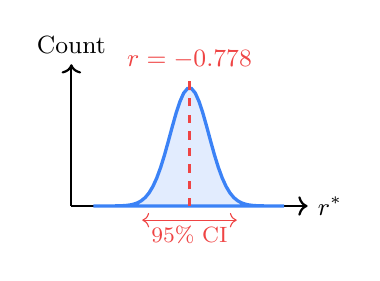
\begin{tikzpicture}[scale=0.6]
  \draw[->, thick] (0,0) -- (5,0) node[right] {\small $r^*$};
  \draw[->, thick] (0,0) -- (0,3) node[above] {\small Count};
  \draw[accent, very thick, domain=0.5:4.5, samples=50, fill=accent!15] plot (\x, {2.5*exp(-3*(\x-2.5)*(\x-2.5))}) -- (4.5,0) -- (0.5,0) -- cycle;
  \draw[softred, thick, dashed] (2.5, 0) -- (2.5, 2.7);
  \node[softred, above] at (2.5, 2.7) {\small $r = -0.778$};
  \draw[<->, softred] (1.5, -0.3) -- (3.5, -0.3);
  \node[softred, font=\footnotesize] at (2.5, -0.6) {95\% CI};
\end{tikzpicture}

\vspace{0.2em}
\footnotesize No formula needed!\\Bootstrap handles any statistic
\end{columns}
\end{frame}


\begin{frame}{Bootstrap for Median: No Formula Exists!}

\textbf{The bootstrap shines when no formula is available}

\begin{columns}
\column{0.5\textwidth}
\textbf{Boston data:}

Median home value: \$21,200

\vspace{0.3em}
\textbf{SE of the median?}

No closed-form formula!

\vspace{0.3em}
\textbf{Bootstrap} ($B = 1000$):

$\text{SE}_B(\text{median}) = \$0.38\text{k}$

95\% CI: $[\$20.5\text{k}, \; \$22.0\text{k}]$

\column{0.45\textwidth}
\textbf{Compare with mean:}

Mean home value: \$22,533

Formula SE: $\$0.41\text{k}$

Bootstrap SE: $\$0.41\text{k}$

\vspace{0.3em}
For the mean: formula and bootstrap agree (as expected)

For the median: \textbf{only bootstrap works}

\vspace{0.3em}
\textcolor{accent}{\textit{Bootstrap is universal!}}
\end{columns}
\end{frame}


\begin{frame}{Think About It: Why $k = n$ Has High Variance}
\begin{columns}
\column{0.55\textwidth}
\textbf{LOOCV:} average $n$ estimates

Each trained on $n-1$ observations

$\Rightarrow$ Training sets differ by only 1 point!

$\Rightarrow$ $\text{MSE}_1, \text{MSE}_2, \ldots, \text{MSE}_n$ are highly \textbf{correlated}

\vspace{0.5em}
\textbf{Recall:}

$\text{Var}(\bar{X}) = \frac{\sigma^2}{n} + \frac{n-1}{n}\rho\sigma^2$

When $\rho$ is large, variance of the average is large!

\column{0.4\textwidth}
\textbf{$k = 10$:} average 10 estimates

Each trained on 90\% of data

Training sets overlap less

$\Rightarrow$ $\text{MSE}_1, \ldots, \text{MSE}_{10}$ are less correlated

$\Rightarrow$ Lower variance of the average

\vspace{0.5em}
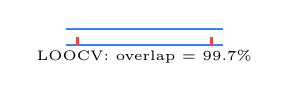
\begin{tikzpicture}[scale=0.5]
  \draw[accent, thick] (0,0) -- (4,0);
  \draw[accent, thick] (0,0.4) -- (4,0.4);
  \draw[softred, very thick, dashed] (0.3, 0) -- (0.3, 0.4);
  \draw[softred, very thick, dashed] (3.7, 0) -- (3.7, 0.4);
  \node[font=\tiny] at (2, -0.3) {LOOCV: overlap = 99.7\%};
\end{tikzpicture}

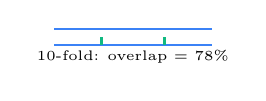
\begin{tikzpicture}[scale=0.5]
  \draw[accent, thick] (0,0) -- (4,0);
  \draw[accent, thick] (0,0.4) -- (4,0.4);
  \draw[softgreen, very thick, dashed] (1.2, 0) -- (1.2, 0.4);
  \draw[softgreen, very thick, dashed] (2.8, 0) -- (2.8, 0.4);
  \node[font=\tiny] at (2, -0.3) {10-fold: overlap = 78\%};
\end{tikzpicture}
\end{columns}
\end{frame}


\begin{frame}{The Cross-Validation Cycle: A Visual Summary}

\begin{center}
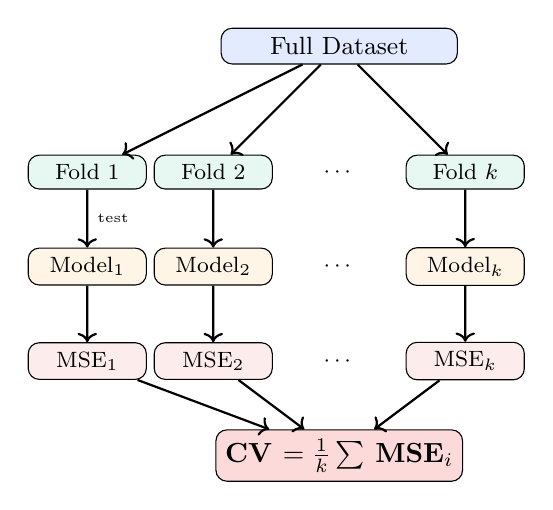
\begin{tikzpicture}[scale=0.8, every node/.style={font=\small}]
  % Data
  \node[draw, fill=accent!15, rounded corners, minimum width=3cm] (data) at (0,3) {Full Dataset};

  % Folds
  \node[draw, fill=softgreen!10, rounded corners, minimum width=1.5cm, font=\footnotesize] (f1) at (-4,1) {Fold 1};
  \node[draw, fill=softgreen!10, rounded corners, minimum width=1.5cm, font=\footnotesize] (f2) at (-2,1) {Fold 2};
  \node[font=\footnotesize] at (0,1) {$\cdots$};
  \node[draw, fill=softgreen!10, rounded corners, minimum width=1.5cm, font=\footnotesize] (fk) at (2,1) {Fold $k$};

  % Models
  \node[draw, fill=amber!10, rounded corners, minimum width=1.5cm, font=\footnotesize] (m1) at (-4,-0.5) {Model$_1$};
  \node[draw, fill=amber!10, rounded corners, minimum width=1.5cm, font=\footnotesize] (m2) at (-2,-0.5) {Model$_2$};
  \node[font=\footnotesize] at (0,-0.5) {$\cdots$};
  \node[draw, fill=amber!10, rounded corners, minimum width=1.5cm, font=\footnotesize] (mk) at (2,-0.5) {Model$_k$};

  % Errors
  \node[draw, fill=softred!10, rounded corners, minimum width=1.5cm, font=\footnotesize] (e1) at (-4,-2) {MSE$_1$};
  \node[draw, fill=softred!10, rounded corners, minimum width=1.5cm, font=\footnotesize] (e2) at (-2,-2) {MSE$_2$};
  \node[font=\footnotesize] at (0,-2) {$\cdots$};
  \node[draw, fill=softred!10, rounded corners, minimum width=1.5cm, font=\footnotesize] (ek) at (2,-2) {MSE$_k$};

  % Final
  \node[draw, fill=softred!20, rounded corners, minimum width=3cm, font=\bfseries] (cv) at (0,-3.5) {CV $= \frac{1}{k}\sum$ MSE$_i$};

  \draw[->, thick] (data) -- (f1);
  \draw[->, thick] (data) -- (f2);
  \draw[->, thick] (data) -- (fk);

  \draw[->, thick] (f1) -- (m1) node[midway, right, font=\tiny] {test};
  \draw[->, thick] (f2) -- (m2);
  \draw[->, thick] (fk) -- (mk);

  \draw[->, thick] (m1) -- (e1);
  \draw[->, thick] (m2) -- (e2);
  \draw[->, thick] (mk) -- (ek);

  \draw[->, thick] (e1) -- (cv);
  \draw[->, thick] (e2) -- (cv);
  \draw[->, thick] (ek) -- (cv);
\end{tikzpicture}
\end{center}
\end{frame}
\begin{frame}{Worked Example: 5-Fold CV by Hand}

\textbf{Data:} 10 observations, 5-fold CV

\begin{columns}
\column{0.48\textwidth}
\begin{tabular}{cccc}
\toprule
Fold & Train & Test & MSE$_i$ \\
\midrule
1 & obs 3--10 & obs 1--2 & 2.1 \\
2 & obs 1,2,5--10 & obs 3--4 & 1.8 \\
3 & obs 1--4,7--10 & obs 5--6 & 2.5 \\
4 & obs 1--6,9--10 & obs 7--8 & 1.9 \\
5 & obs 1--8 & obs 9--10 & 2.3 \\
\bottomrule
\end{tabular}

\column{0.48\textwidth}
$$\text{CV}_{(5)} = \frac{2.1 + 1.8 + 2.5 + 1.9 + 2.3}{5}$$

$$= \frac{10.6}{5} = 2.12$$

\vspace{0.5em}
Each observation appears in the test set \textbf{exactly once}

Every observation contributes to the error estimate
\end{columns}
\end{frame}


\begin{frame}{The LOOCV Shortcut: Why It Works}

$$\text{CV}_{(n)} = \frac{1}{n}\sum_{i=1}^{n}\left(\frac{e_i}{1-h_i}\right)^2$$

\begin{columns}
\column{0.55\textwidth}
\textbf{Intuition:}

$e_i = y_i - \hat{y}_i$ = ordinary residual

$h_i$ = leverage of observation $i$

\vspace{0.3em}
High leverage $\Rightarrow$ observation strongly influences its own fit

$\Rightarrow$ Ordinary residual \textbf{underestimates} how much this point deviates

$\Rightarrow$ Dividing by $(1-h_i)$ \textbf{corrects} this

\column{0.4\textwidth}
\textbf{Numerical check:}

\vspace{0.3em}
\begin{tabular}{cccc}
\toprule
$i$ & $e_i$ & $h_i$ & $\frac{e_i}{1-h_i}$ \\
\midrule
1 & 0.5 & 0.05 & 0.53 \\
2 & $-0.8$ & 0.02 & $-0.82$ \\
3 & 1.2 & 0.15 & 1.41 \\
4 & $-0.3$ & 0.30 & $-0.43$ \\
\bottomrule
\end{tabular}

\vspace{0.3em}
Obs 4: high leverage $\Rightarrow$ big correction
\end{columns}
\end{frame}


\begin{frame}{CV for Choosing the Right Polynomial Degree}
\begin{columns}
\column{0.5\textwidth}
\textbf{Auto data: 10-fold CV}

\begin{tabular}{cc}
\toprule
Degree & CV MSE \\
\midrule
1 (linear) & 24.27 \\
\textcolor{softgreen}{2 (quadratic)} & \textcolor{softgreen}{19.27} \\
3 (cubic) & 19.35 \\
4 & 19.29 \\
5 & 19.03 \\
\bottomrule
\end{tabular}

\vspace{0.3em}
\textbf{Conclusion:} Quadratic is sufficient

Higher degrees add complexity\\
without meaningful improvement

\column{0.45\textwidth}
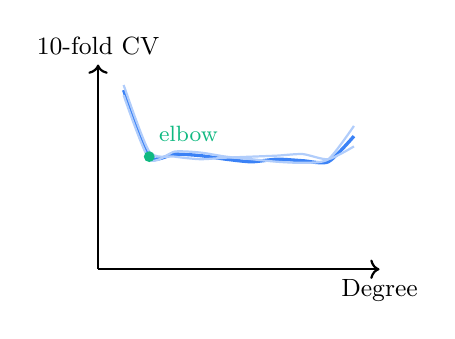
\begin{tikzpicture}[scale=0.65]
  \draw[->, thick] (0,0) -- (5.5,0) node[below] {\small Degree};
  \draw[->, thick] (0,0) -- (0,4) node[above] {\small 10-fold CV};
  % Multiple 10-fold curves
  \draw[accent, very thick, smooth, tension=0.4] plot coordinates {(0.5,3.5)(1,2.2)(1.5,2.25)(2,2.22)(2.5,2.15)(3,2.10)(3.5,2.15)(4,2.12)(4.5,2.10)(5,2.6)};
  \draw[accent!40, thick, smooth, tension=0.4] plot coordinates {(0.5,3.6)(1,2.3)(1.5,2.20)(2,2.15)(2.5,2.18)(3,2.20)(3.5,2.22)(4,2.25)(4.5,2.15)(5,2.4)};
  \draw[accent!40, thick, smooth, tension=0.4] plot coordinates {(0.5,3.4)(1,2.15)(1.5,2.30)(2,2.28)(2.5,2.20)(3,2.15)(3.5,2.10)(4,2.08)(4.5,2.15)(5,2.8)};
  \fill[softgreen] (1, 2.2) circle (3pt);
  \node[softgreen, above right, font=\footnotesize] at (1, 2.3) {elbow};
\end{tikzpicture}

\vspace{0.3em}
\footnotesize 9 different random splits\\of 10-fold CV all agree!
\end{columns}
\end{frame}


\begin{frame}{Bootstrap Confidence Intervals}

\textbf{Two common approaches:}

\vspace{0.3em}
\begin{columns}
\column{0.48\textwidth}
\textbf{Normal bootstrap CI:}

$$\hat{\theta} \pm z_{\alpha/2} \cdot \text{SE}_B(\hat{\theta})$$

Assumes $\hat{\theta}$ is approximately normal

Simple but can be inaccurate

\vspace{0.3em}
\textbf{Example:}

$\hat{\alpha} \pm 1.96 \times 0.089$

$= [0.40, \; 0.75]$

\column{0.48\textwidth}
\textbf{Percentile bootstrap CI:}

Use the $\alpha/2$ and $1-\alpha/2$ quantiles of\\
the bootstrap distribution directly

\vspace{0.3em}
No normality assumption!

\vspace{0.3em}
\textbf{Example:}

2.5th percentile: 0.39

97.5th percentile: 0.74

$\Rightarrow$ 95\% CI: $[0.39, \; 0.74]$
\end{columns}
\end{frame}


\begin{frame}{Common Mistakes with CV}
\begin{enumerate}
  \item \textbf{Data leakage:} Preprocessing \textit{before} splitting
  \begin{itemize}
    \item[$\circ$] \textcolor{softred}{Wrong:} Standardize all data, then split into folds
    \item[$\circ$] \textcolor{softgreen}{Right:} Standardize training folds only, apply to test fold
  \end{itemize}

  \vspace{0.3em}
  \item \textbf{Using CV error as the final test error}
  \begin{itemize}
    \item[$\circ$] CV is for model \textbf{selection}, not final assessment
    \item[$\circ$] Ideally, hold out a separate test set that is never touched during CV
  \end{itemize}

  \vspace{0.3em}
  \item \textbf{Forgetting to refit after CV}
  \begin{itemize}
    \item[$\circ$] After choosing the best model via CV, refit on \textbf{all} data
  \end{itemize}

  \vspace{0.3em}
  \item \textbf{Too few folds with small $n$}
  \begin{itemize}
    \item[$\circ$] $k = 10$ with $n = 30$ $\Rightarrow$ only 3 test obs per fold $\Rightarrow$ noisy
  \end{itemize}
\end{enumerate}
\end{frame}


\begin{frame}{Bootstrap vs.\ Cross-Validation: Different Questions}

\begin{center}
\begin{tabular}{lcc}
\toprule
 & Cross-Validation & Bootstrap \\
\midrule
Purpose & Estimate \textbf{test error} & Estimate \textbf{uncertainty} \\
Question & How well does model predict? & How variable is $\hat{\theta}$? \\
Resampling & Split into folds (no replacement) & Sample with replacement \\
Output & CV error (MSE or error rate) & SE($\hat{\theta}$) or CI \\
Use for & Model selection, tuning & Confidence intervals, SEs \\
\bottomrule
\end{tabular}
\end{center}

\vspace{0.5em}
\textbf{Both are resampling methods, but they answer different questions!}

\vspace{0.3em}
\textit{CV: ``Which model is best?'' \quad Bootstrap: ``How sure are we?''}
\end{frame}


\begin{frame}{The Bootstrap in Pictures}

\begin{center}
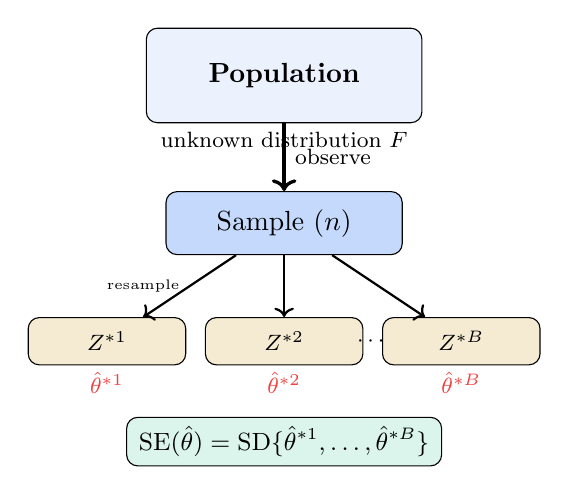
\begin{tikzpicture}[scale=0.75]
  % Population
  \node[draw, fill=accent!10, rounded corners, minimum width=3.5cm, minimum height=1.2cm] (pop) at (0, 5) {\textbf{Population}};
  \node[below, font=\footnotesize] at (0, 4.2) {unknown distribution $F$};

  % Sample
  \node[draw, fill=accent!30, rounded corners, minimum width=3cm, minimum height=0.8cm] (samp) at (0, 2.5) {Sample ($n$)};
  \draw[->, very thick] (pop) -- (samp) node[midway, right, font=\footnotesize] {observe};

  % Bootstrap samples
  \node[draw, fill=beige, rounded corners, minimum width=2cm, minimum height=0.6cm, font=\footnotesize] (b1) at (-3, 0.5) {$Z^{*1}$};
  \node[draw, fill=beige, rounded corners, minimum width=2cm, minimum height=0.6cm, font=\footnotesize] (b2) at (0, 0.5) {$Z^{*2}$};
  \node[font=\footnotesize] at (1.5, 0.5) {$\cdots$};
  \node[draw, fill=beige, rounded corners, minimum width=2cm, minimum height=0.6cm, font=\footnotesize] (bB) at (3, 0.5) {$Z^{*B}$};
  \draw[->, thick] (samp) -- (b1) node[midway, left, font=\tiny] {resample};
  \draw[->, thick] (samp) -- (b2);
  \draw[->, thick] (samp) -- (bB);

  % Estimates
  \node[softred, font=\footnotesize] at (-3, -0.2) {$\hat{\theta}^{*1}$};
  \node[softred, font=\footnotesize] at (0, -0.2) {$\hat{\theta}^{*2}$};
  \node[softred, font=\footnotesize] at (3, -0.2) {$\hat{\theta}^{*B}$};

  % Final
  \node[draw, fill=softgreen!15, rounded corners, minimum width=4cm, font=\small] at (0, -1.2) {$\text{SE}(\hat{\theta}) = \text{SD}\{\hat{\theta}^{*1}, \ldots, \hat{\theta}^{*B}\}$};
\end{tikzpicture}
\end{center}
\end{frame}


\begin{frame}{Quick Quiz: Test Yourself!}
\begin{enumerate}
  \item LOOCV trains on how many observations each time?
  \pause
  \item[]{\textcolor{muted}{\footnotesize $n-1$ observations (leaves out exactly 1)}}

  \vspace{0.3em}
  \item In 10-fold CV, what fraction of data is used for training in each fold?
  \pause
  \item[]{\textcolor{muted}{\footnotesize $9/10 = 90\%$}}

  \vspace{0.3em}
  \item Why does LOOCV have higher variance than 10-fold CV?
  \pause
  \item[]{\textcolor{muted}{\footnotesize Training sets overlap almost completely $\Rightarrow$ estimates are highly correlated}}

  \vspace{0.3em}
  \item What does the bootstrap sample \textbf{with} or \textbf{without} replacement?
  \pause
  \item[]{\textcolor{muted}{\footnotesize \textbf{With} replacement --- that's the key idea!}}
\end{enumerate}
\end{frame}


\begin{frame}{Quick Quiz: More Questions}
\begin{enumerate}
  \setcounter{enumi}{4}
  \item What fraction of observations is NOT in a bootstrap sample (on average)?
  \pause
  \item[]{\textcolor{muted}{\footnotesize $\approx 36.8\%$ (out-of-bag observations)}}

  \vspace{0.3em}
  \item Can you use cross-validation with logistic regression?
  \pause
  \item[]{\textcolor{muted}{\footnotesize Yes! Use misclassification rate instead of MSE}}

  \vspace{0.3em}
  \item LOOCV on Auto gives MSE $=24.23$ for linear, $19.25$ for quadratic. Which model?
  \pause
  \item[]{\textcolor{muted}{\footnotesize Quadratic --- lower CV error, big improvement over linear}}

  \vspace{0.3em}
  \item After selecting a model via CV, should you report the CV error as test error?
  \pause
  \item[]{\textcolor{muted}{\footnotesize Ideally no --- CV was used for selection, use a held-out test set for final assessment}}
\end{enumerate}
\end{frame}


\begin{frame}{R Functions: Quick Reference}

\begin{center}
\begin{tabular}{ll}
\toprule
\textbf{Cross-Validation} & \\
\midrule
\texttt{cv.glm(data, glmfit)} & LOOCV (default) \\
\texttt{cv.glm(data, glmfit, K=10)} & 10-fold CV \\
\texttt{cv.glm()\$delta[1]} & Raw CV error \\
\texttt{cv.glm()\$delta[2]} & Bias-corrected CV error \\
\bottomrule
\end{tabular}
\end{center}

\vspace{0.3em}
\begin{center}
\begin{tabular}{ll}
\toprule
\textbf{Bootstrap} & \\
\midrule
\texttt{boot(data, statistic, R=1000)} & Run $R$ bootstrap replicates \\
\texttt{boot.out\$t0} & Original estimate \\
\texttt{boot.out\$t} & Matrix of bootstrap estimates \\
\texttt{boot.ci(boot.out)} & Bootstrap confidence intervals \\
\bottomrule
\end{tabular}
\end{center}

\vspace{0.3em}
\footnotesize Both from the \texttt{boot} package: \texttt{library(boot)}
\end{frame}


\begin{frame}{Key Formulas: Cheat Sheet}
\begin{columns}
\column{0.48\textwidth}
\textbf{Cross-Validation:}
\begin{align*}
\text{CV}_{(k)} &= \frac{1}{k}\sum_{i=1}^{k}\text{MSE}_i \\[4pt]
\text{CV}_{(n)} &= \frac{1}{n}\sum_{i=1}^{n}\left(\frac{e_i}{1-h_i}\right)^2
\end{align*}

Classification:
$$\text{CV}_{(k)} = \frac{1}{k}\sum_{i=1}^{k}\text{Err}_i$$

\column{0.48\textwidth}
\textbf{Bootstrap:}
$$\text{SE}_B(\hat{\theta}) = \sqrt{\frac{1}{B-1}\sum_{b=1}^B (\hat{\theta}^{*b} - \bar{\hat{\theta}}^*)^2}$$

\vspace{0.3em}
Out-of-bag probability:
$$P(\text{not selected}) = \left(1-\frac{1}{n}\right)^n \approx e^{-1}$$

\vspace{0.3em}
Normal bootstrap CI:
$$\hat{\theta} \pm z_{\alpha/2} \cdot \text{SE}_B$$
\end{columns}
\end{frame}


\begin{frame}{Summary: Chapter 5}
\begin{columns}
\column{0.48\textwidth}
\textbf{Cross-Validation:}
\begin{itemize}
  \item Estimates test error without a test set
  \item Validation set: simple but high variance
  \item LOOCV: low bias, high variance, expensive
  \item $k$-fold: best bias-variance balance at $k=5$--$10$
  \item Use for model selection and tuning
\end{itemize}

\column{0.48\textwidth}
\textbf{Bootstrap:}
\begin{itemize}
  \item Estimates uncertainty of any statistic
  \item Sample with replacement, $B$ times
  \item No distributional assumptions
  \item Provides SEs and CIs
  \item More honest than formula-based SEs when model assumptions fail
\end{itemize}
\end{columns}

\vspace{0.5em}
\centering
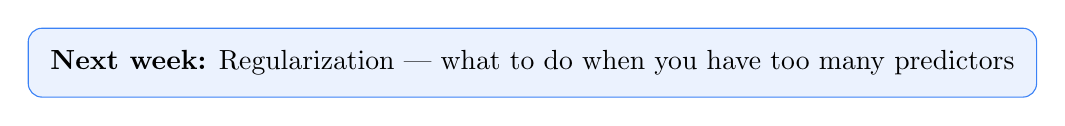
\begin{tikzpicture}
\node[fill=accent!10, rounded corners=5pt, inner sep=8pt, draw=accent] {
  \textbf{Next week:} Regularization --- what to do when you have too many predictors
};
\end{tikzpicture}
\end{frame}


\begin{frame}{Implementing CV Manually in R}
\begin{columns}
\column{0.55\textwidth}
\footnotesize
\texttt{set.seed(1)}\\
\texttt{k <- 10}\\
\texttt{n <- nrow(Auto)}\\
\texttt{folds <- sample(rep(1:k, length=n))}\\
\texttt{cv\_errors <- rep(0, k)}\\
\texttt{}\\
\texttt{for (i in 1:k) \{}\\
\texttt{\quad test\_idx <- which(folds == i)}\\
\texttt{\quad fit <- lm(mpg \textasciitilde{} poly(hp,2),}\\
\texttt{\quad\quad\quad\quad data=Auto[-test\_idx,])}\\
\texttt{\quad pred <- predict(fit, Auto[test\_idx,])}\\
\texttt{\quad cv\_errors[i] <- mean(}\\
\texttt{\quad\quad (Auto\$mpg[test\_idx] - pred)\^{}2)}\\
\texttt{\}}\\
\texttt{mean(cv\_errors)  \# CV estimate}
\normalsize

\column{0.4\textwidth}
\textbf{Key steps:}

\begin{enumerate}
  \item Create fold assignments
  \item Loop over folds
  \item Train on $-$fold, test on fold
  \item Average MSEs
\end{enumerate}

\vspace{0.3em}
\textit{Understanding the mechanics helps you debug and customize!}

\vspace{0.3em}
\textbf{Or use:}\\
\texttt{cv.glm(data, fit, K=10)}
\end{columns}
\end{frame}


\begin{frame}{Implementing Bootstrap Manually in R}
\begin{columns}
\column{0.55\textwidth}
\footnotesize
\texttt{B <- 1000}\\
\texttt{n <- nrow(Auto)}\\
\texttt{beta1\_boot <- rep(0, B)}\\
\texttt{}\\
\texttt{for (b in 1:B) \{}\\
\texttt{\quad idx <- sample(n, replace=TRUE)}\\
\texttt{\quad fit <- lm(mpg \textasciitilde{} horsepower,}\\
\texttt{\quad\quad\quad\quad data=Auto[idx,])}\\
\texttt{\quad beta1\_boot[b] <- coef(fit)[2]}\\
\texttt{\}}\\
\texttt{}\\
\texttt{sd(beta1\_boot)  \# bootstrap SE}\\
\texttt{quantile(beta1\_boot, c(.025,.975))}
\normalsize

\column{0.4\textwidth}
\textbf{Key:} \texttt{replace = TRUE}

This is what makes it bootstrap!

\vspace{0.5em}
\textbf{Results:}

$\text{SE}_B(\hat{\beta}_1) \approx 0.007$

95\% CI: $[-0.172, -0.144]$

\vspace{0.3em}
\textbf{Or use:}\\
\texttt{boot(data, statistic, R=1000)}
\end{columns}
\end{frame}


\begin{frame}{The \texttt{boot()} Function: Anatomy}

\textbf{Three ingredients:}

\begin{enumerate}
  \item \textbf{Data:} The original dataset
  \item \textbf{Statistic:} A function that takes (data, index) and returns $\hat{\theta}$
  \item \textbf{R:} Number of bootstrap replicates
\end{enumerate}

\vspace{0.3em}
\begin{columns}
\column{0.48\textwidth}
\textbf{The statistic function:}
\footnotesize
\texttt{my.fn <- function(data, index) \{}\\
\texttt{\quad d <- data[index, ]}\\
\texttt{\quad fit <- lm(mpg \textasciitilde{} hp, data=d)}\\
\texttt{\quad return(coef(fit))}\\
\texttt{\}}
\normalsize

\vspace{0.3em}
\texttt{index} = vector of row indices

\texttt{boot()} generates these with replacement

\column{0.48\textwidth}
\textbf{Running it:}
\footnotesize
\texttt{library(boot)}\\
\texttt{result <- boot(Auto, my.fn, R=1000)}\\
\texttt{result\$t0}  \textit{\# original estimate}\\
\texttt{result\$t}   \textit{\# B x p matrix}\\
\texttt{boot.ci(result)}  \textit{\# CIs}
\normalsize

\vspace{0.3em}
\texttt{t0} = $\hat{\theta}$ from original data

\texttt{t} = all $B$ bootstrap estimates
\end{columns}
\end{frame}


\begin{frame}{Visualizing Bootstrap Distributions}

\begin{center}
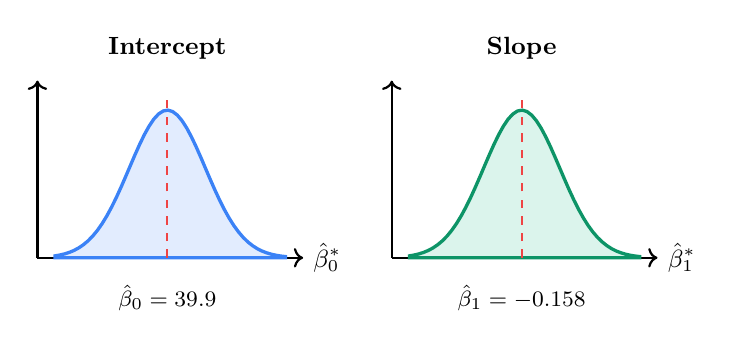
\begin{tikzpicture}[scale=0.75]
  % Beta_0
  \begin{scope}[xshift=0cm]
    \draw[->, thick] (0,0) -- (4.5,0) node[right] {\small $\hat{\beta}_0^*$};
    \draw[->, thick] (0,0) -- (0,3);
    \draw[accent, very thick, domain=0.3:4.2, samples=50, fill=accent!15] plot (\x, {2.5*exp(-1.2*(\x-2.2)*(\x-2.2))}) -- (4.2,0) -- (0.3,0) -- cycle;
    \draw[softred, thick, dashed] (2.2, 0) -- (2.2, 2.7);
    \node[below, font=\footnotesize] at (2.2, -0.3) {$\hat{\beta}_0 = 39.9$};
    \node[above, font=\small\bfseries] at (2.2, 3.2) {Intercept};
  \end{scope}

  % Beta_1
  \begin{scope}[xshift=6cm]
    \draw[->, thick] (0,0) -- (4.5,0) node[right] {\small $\hat{\beta}_1^*$};
    \draw[->, thick] (0,0) -- (0,3);
    \draw[softgreen!80!black, very thick, domain=0.3:4.2, samples=50, fill=softgreen!15] plot (\x, {2.5*exp(-1.2*(\x-2.2)*(\x-2.2))}) -- (4.2,0) -- (0.3,0) -- cycle;
    \draw[softred, thick, dashed] (2.2, 0) -- (2.2, 2.7);
    \node[below, font=\footnotesize] at (2.2, -0.3) {$\hat{\beta}_1 = -0.158$};
    \node[above, font=\small\bfseries] at (2.2, 3.2) {Slope};
  \end{scope}
\end{tikzpicture}
\end{center}

\vspace{0.3em}
\begin{itemize}
  \item Both distributions are approximately normal $\Rightarrow$ normal CI is fine
  \item Width of histogram $\propto$ SE
  \item The intercept has wider spread (larger SE) than the slope
\end{itemize}
\end{frame}


\begin{frame}{CV for Choosing Between Methods (Not Just Tuning)}

\textbf{Question:} Linear regression or KNN for predicting mpg?

\vspace{0.3em}
\begin{columns}
\column{0.48\textwidth}
\textbf{10-fold CV:}

\begin{tabular}{lc}
\toprule
Method & CV MSE \\
\midrule
lm(mpg $\sim$ hp) & 24.3 \\
lm(mpg $\sim$ poly(hp,2)) & 19.3 \\
KNN $K=5$ & 20.1 \\
KNN $K=10$ & 20.8 \\
KNN $K=20$ & 22.5 \\
\textcolor{softgreen}{lm(mpg $\sim$ wt+yr+orig)} & \textcolor{softgreen}{12.6} \\
\bottomrule
\end{tabular}

\column{0.48\textwidth}
\textbf{Conclusion:}

Linear regression with the right predictors beats KNN!

\vspace{0.3em}
\textbf{Why?}

\begin{itemize}
  \item The relationship is approximately linear
  \item KNN suffers from curse of dimensionality
  \item Linear model uses structure effectively
\end{itemize}

\vspace{0.3em}
\textit{CV lets us compare apples to oranges fairly!}
\end{columns}
\end{frame}


\begin{frame}{Double Use of Data: A Subtle Error}

\textbf{Common mistake in practice:}

\begin{columns}
\column{0.48\textwidth}
\textbf{\textcolor{softred}{Wrong:}}

\begin{enumerate}
  \item Look at all data to choose features
  \item Then run CV on those features
  \item Report CV error
\end{enumerate}

\vspace{0.3em}
The feature selection ``saw'' the test data!

$\Rightarrow$ CV error is too optimistic

\column{0.48\textwidth}
\textbf{\textcolor{softgreen}{Right:}}

\begin{enumerate}
  \item Split into folds
  \item \textbf{Inside each fold:}
  \begin{enumerate}
    \item Select features on train
    \item Fit model on train
    \item Test on held-out fold
  \end{enumerate}
\end{enumerate}

\vspace{0.3em}
Feature selection is part of the model-building pipeline --- it must be inside CV!
\end{columns}

\vspace{0.3em}
\centering
\fbox{\parbox{0.65\textwidth}{\centering \textbf{Golden rule:} Everything that uses data to make decisions must be \textbf{inside} the CV loop}}
\end{frame}


\begin{frame}{LOOCV for Classification: Worked Example}

\textbf{Default data:} $n = 10{,}000$, logistic regression

\vspace{0.3em}
\begin{columns}
\column{0.5\textwidth}
\textbf{Iteration $i = 1$:}

Train on obs $\{2, 3, \ldots, 10000\}$

Predict obs 1: $\hat{p}_1 = 0.02$

Actual: default = No

$\Rightarrow$ $\text{Err}_1 = \mathbf{1}(\text{No} \neq \text{No}) = 0$ \textcolor{softgreen}{\checkmark}

\vspace{0.3em}
\textbf{Iteration $i = 47$:}

Train without obs 47

Predict: $\hat{p}_{47} = 0.62$

Actual: default = No

$\Rightarrow$ $\text{Err}_{47} = \mathbf{1}(\text{Yes} \neq \text{No}) = 1$ \textcolor{softred}{$\times$}

\column{0.45\textwidth}
\textbf{After all $n$ iterations:}

$$\text{CV}_{(n)} = \frac{1}{10000}\sum_{i=1}^{10000}\text{Err}_i$$

$= \frac{264}{10000} = 2.64\%$

\vspace{0.5em}
264 observations were misclassified when left out

\vspace{0.3em}
\footnotesize For logistic, LOOCV shortcut doesn't apply --- must refit $n$ times (slow!)

Better: use 10-fold CV
\end{columns}
\end{frame}


\begin{frame}{Sample Size and CV Stability}
\begin{columns}
\column{0.5\textwidth}
\textbf{How stable is 10-fold CV?}

\vspace{0.3em}
Run 10-fold CV 100 times with different random folds:

\begin{tabular}{ccc}
\toprule
$n$ & Mean CV & SD of CV \\
\midrule
50 & 22.3 & 3.1 \\
100 & 20.8 & 1.8 \\
200 & 19.5 & 0.9 \\
392 & 19.3 & 0.4 \\
\bottomrule
\end{tabular}

\column{0.45\textwidth}
\textbf{Key insight:}

Larger $n$ $\Rightarrow$ more stable CV estimates

\vspace{0.3em}
With $n = 50$: CV varies a lot (SD $= 3.1$)

With $n = 392$: very stable (SD $= 0.4$)

\vspace{0.5em}
\textit{Small datasets: consider LOOCV\\or repeated CV for more stable\\estimates}
\end{columns}
\end{frame}


\begin{frame}{Bootstrap: Estimating SE of Any Statistic}

\textbf{The bootstrap works for ANY computable statistic!}

\vspace{0.5em}
\begin{center}
\begin{tabular}{lcc}
\toprule
Statistic & Formula SE exists? & Bootstrap works? \\
\midrule
Mean $\bar{X}$ & \textcolor{softgreen}{Yes} ($s/\sqrt{n}$) & \textcolor{softgreen}{Yes} \\
Regression $\hat{\beta}$ & \textcolor{softgreen}{Yes} (under assumptions) & \textcolor{softgreen}{Yes} \\
Median & \textcolor{softred}{No simple formula} & \textcolor{softgreen}{Yes} \\
Correlation $r$ & Complex (Fisher's $z$) & \textcolor{softgreen}{Yes} \\
Ratio $\bar{X}/\bar{Y}$ & \textcolor{softred}{No} & \textcolor{softgreen}{Yes} \\
90th percentile & \textcolor{softred}{No} & \textcolor{softgreen}{Yes} \\
Custom $\hat{\alpha}$ & \textcolor{softred}{No} & \textcolor{softgreen}{Yes} \\
\bottomrule
\end{tabular}
\end{center}

\vspace{0.3em}
\centering
\textcolor{accent}{\textbf{The bootstrap is universal --- that's its superpower}}
\end{frame}


\begin{frame}{Residual Bootstrap vs.\ Pairs Bootstrap}
\begin{columns}
\column{0.48\textwidth}
\textbf{Pairs bootstrap} (standard):

Resample $(x_i, y_i)$ pairs together

$\{(x_3, y_3), (x_1, y_1), (x_3, y_3), \ldots\}$

\vspace{0.3em}
\begin{itemize}
  \item[\textcolor{softgreen}{\textbullet}] No model assumptions
  \item[\textcolor{softgreen}{\textbullet}] Handles heteroscedasticity
  \item[\textcolor{softred}{\textbullet}] May change leverage structure
\end{itemize}

\column{0.48\textwidth}
\textbf{Residual bootstrap:}

\begin{enumerate}
  \item Fit model: $\hat{y}_i = \hat{\beta}_0 + \hat{\beta}_1 x_i$
  \item Compute residuals: $e_i = y_i - \hat{y}_i$
  \item Resample residuals: $e^*$
  \item New data: $y_i^* = \hat{y}_i + e_i^*$
  \item Refit on $(x_i, y_i^*)$
\end{enumerate}

\vspace{0.3em}
\begin{itemize}
  \item[\textcolor{softgreen}{\textbullet}] Preserves $X$ structure
  \item[\textcolor{softred}{\textbullet}] Assumes constant variance
\end{itemize}
\end{columns}

\vspace{0.3em}
\centering
\textit{In practice, pairs bootstrap is more common --- safer and simpler}
\end{frame}


\begin{frame}{Connecting CV to Weeks 4--10}
\begin{columns}
\column{0.55\textwidth}
\textbf{CV will be used in every remaining week:}

\begin{tabular}{ll}
\toprule
Week & CV used for \\
\midrule
4 & Choose $\lambda$ in Lasso/Ridge \\
5 & Choose \# knots in splines \\
6 & Estimate RF test error \\
7 & Tune boosting parameters \\
8 & Choose cost $C$ in SVM \\
9 & Early stopping in neural nets \\
10 & Choose \# clusters \\
\bottomrule
\end{tabular}

\column{0.4\textwidth}
\textbf{The bootstrap too:}

\begin{itemize}
  \item Week 6: Out-of-bag error in Random Forests
  \item Week 7: Bagging = bootstrap aggregation
  \item Confidence intervals everywhere
\end{itemize}

\vspace{0.5em}
\centering
\fbox{\parbox{3cm}{\centering \textit{Today's methods are\\the foundation for\\everything ahead}}}
\end{columns}
\end{frame}


\begin{frame}{Quick Quiz: Advanced Questions}
\begin{enumerate}
  \item What is the ``one standard error rule'' and when do you use it?
  \pause
  \item[]{\textcolor{muted}{\footnotesize Choose the simplest model within 1 SE of the minimum CV error --- for parsimony}}

  \vspace{0.3em}
  \item You run 10-fold CV and get MSE $= 15.2$. Is this the expected test MSE?
  \pause
  \item[]{\textcolor{muted}{\footnotesize Approximately yes, but it has some bias (slightly overestimates true test error)}}

  \vspace{0.3em}
  \item Can you bootstrap a neural network? Is it practical?
  \pause
  \item[]{\textcolor{muted}{\footnotesize Yes in principle, but each refit takes hours $\Rightarrow$ impractical. Use dropout instead.}}

  \vspace{0.3em}
  \item Why should feature selection happen INSIDE the CV loop?
  \pause
  \item[]{\textcolor{muted}{\footnotesize Otherwise the test fold ``leaks'' into the selection step $\Rightarrow$ optimistic CV error}}
\end{enumerate}
\end{frame}


% ═══════════ EXERCISES ═══════════
\begin{frame}{Exercise 1: Validation Set on Default (ISLR 5.4 Q5)}

\textbf{Data:} \texttt{Default} \hfill Logistic: \texttt{default \textasciitilde{} income + balance}

\begin{enumerate}
  \item Fit logistic on full data
  \item Split into train/validation, fit on train, compute validation error
  \item Repeat 3 times with different seeds --- how much does error vary?
  \item Add \texttt{student} --- does validation error improve?
\end{enumerate}

\fbox{\textbf{Key insight:} Error varies $\pm 0.5\%$ across splits}
\end{frame}


\begin{frame}{Exercise 2: Bootstrap SEs for Logistic (ISLR 5.4 Q6)}

\textbf{Data:} \texttt{Default}

\begin{enumerate}
  \item Fit logistic: \texttt{default \textasciitilde{} income + balance}
  \item Compute formula-based SEs from \texttt{summary()}
  \item Write a \texttt{boot.fn()} function that returns coefficients
  \item Use \texttt{boot()} with $B = 1000$ to get bootstrap SEs
  \item Compare formula SEs vs.\ bootstrap SEs
\end{enumerate}
\end{frame}


\begin{frame}{Exercise 3: LOOCV on Auto (ISLR 5.4 Q5-6)}

\textbf{Data:} \texttt{Auto} \hfill \texttt{mpg \textasciitilde{} poly(horsepower, d)}

\begin{enumerate}
  \item Compute LOOCV error for $d = 1, \ldots, 10$
  \item Which degree minimizes LOOCV?
  \item Repeat with 10-fold CV --- same conclusion?
  \item Bootstrap SE for the linear regression coefficients
  \item Compare bootstrap SEs to \texttt{summary()} SEs
\end{enumerate}

\fbox{\textbf{Hint:} \texttt{cv.glm(Auto, glm.fit)\$delta[1]} for LOOCV}
\end{frame}


\begin{frame}{Exercise 4: Bootstrap on Portfolio (ISLR 5.4 Q8)}

\textbf{Data:} \texttt{Portfolio} \hfill Estimate optimal $\alpha$

\begin{enumerate}
  \item Write a function to compute $\hat{\alpha}$ from the formula
  \item Use \texttt{boot()} with $B = 1000$
  \item Report $\hat{\alpha}$ and $\text{SE}_B(\hat{\alpha})$
  \item Construct a 95\% confidence interval
\end{enumerate}
\end{frame}


% ═══════════ SOLUTIONS ═══════════
\begin{frame}{Solution: Exercise 1 --- Validation Set}
\begin{columns}
\column{0.5\textwidth}
\textbf{Three different splits:}

\begin{tabular}{cc}
\toprule
Seed & Validation Error \\
\midrule
1 & 2.6\% \\
42 & 2.8\% \\
123 & 2.4\% \\
\bottomrule
\end{tabular}

\vspace{0.3em}
Error varies by $\sim 0.4\%$

\vspace{0.3em}
Adding \texttt{student}: no meaningful reduction

\column{0.45\textwidth}
\textbf{Key takeaway:}

The validation set approach gives \textbf{variable} results

\vspace{0.3em}
This is why $k$-fold CV is preferred --- it averages over multiple splits

\vspace{0.3em}
\texttt{student} adds nothing beyond \texttt{balance} (as we saw in Week 2)
\end{columns}
\end{frame}


\begin{frame}{Solution: Exercise 3 --- LOOCV on Auto}
\begin{columns}
\column{0.5\textwidth}
\textbf{LOOCV results:}

\begin{tabular}{cc}
\toprule
Degree & LOOCV MSE \\
\midrule
1 & 24.23 \\
\textcolor{softgreen}{2} & \textcolor{softgreen}{19.25} \\
3 & 19.33 \\
5 & 19.03 \\
10 & 19.49 \\
\bottomrule
\end{tabular}

\vspace{0.3em}
\textbf{10-fold CV:} Same conclusion\\
--- quadratic is the elbow

\column{0.45\textwidth}
\textbf{Bootstrap vs.\ Formula SEs:}

\vspace{0.3em}
\begin{tabular}{lcc}
\toprule
 & Formula & Bootstrap \\
\midrule
$\hat{\beta}_0$ & 0.717 & 0.860 \\
$\hat{\beta}_1$ & 0.006 & 0.007 \\
\bottomrule
\end{tabular}

\vspace{0.3em}
Bootstrap SEs are larger

$\Rightarrow$ Formula underestimates uncertainty because true relationship is non-linear
\end{columns}
\end{frame}


\begin{frame}{Solution: Exercise 4 --- Bootstrap on Portfolio}
\begin{columns}
\column{0.5\textwidth}
\textbf{R code outline:}

\vspace{0.2em}
\footnotesize
\texttt{alpha.fn <- function(data, index) \{}

\texttt{\quad X <- data\$X[index]}

\texttt{\quad Y <- data\$Y[index]}

\texttt{\quad (var(Y) - cov(X,Y)) /}

\texttt{\quad (var(X) + var(Y) - 2*cov(X,Y))}

\texttt{\}}

\vspace{0.2em}
\texttt{boot(Portfolio, alpha.fn, R=1000)}
\normalsize

\column{0.45\textwidth}
\textbf{Results:}

$\hat{\alpha} = 0.576$

$\text{SE}_B(\hat{\alpha}) = 0.089$

\vspace{0.3em}
\textbf{95\% CI:}

Normal: $[0.40, \; 0.75]$

Percentile: $[0.39, \; 0.74]$

\vspace{0.3em}
\textit{Invest 58\% in $X$, 42\% in $Y$\\
with substantial uncertainty}
\end{columns}
\end{frame}


% ═══════════ CLOSING ═══════════
\begin{frame}{What's Next?}

\begin{center}
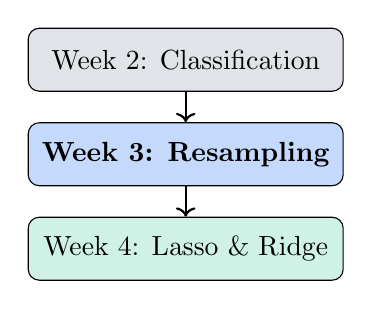
\begin{tikzpicture}[scale=0.8]
  \node[draw, fill=muted!20, rounded corners, minimum width=4cm, minimum height=0.8cm] (w2) at (0,0) {Week 2: Classification};
  \node[draw, fill=accent!30, rounded corners, minimum width=4cm, minimum height=0.8cm, font=\bfseries] (w3) at (0,-1.5) {Week 3: Resampling};
  \node[draw, fill=softgreen!20, rounded corners, minimum width=4cm, minimum height=0.8cm] (w4) at (0,-3.0) {Week 4: Lasso \& Ridge};
  \draw[->, thick] (w2) -- (w3);
  \draw[->, thick] (w3) -- (w4);
\end{tikzpicture}
\end{center}

\vspace{0.3em}
\textbf{Homework:} ISLR Chapter 5: Q5, 6, 7, 8

\textbf{Lab:} \texttt{Lab\_Week03.R} --- CV and Bootstrap on Auto, Default, Portfolio

\textbf{Next week:} Too many predictors? $\Rightarrow$ Lasso \& Ridge Regression!
\end{frame}


\begin{frame}{}
\centering
\vspace{2cm}
{\Huge\textbf{Thank You}}

\vspace{1em}
{\Large Questions?}

\vspace{1.5em}
{\large Dr.\ Endri Ra\c{c}o \quad|\quad Machine Learning with R}

\vspace{0.5em}
{\normalsize \texttt{github.com/endri81/ISLRv2-solutions}}
\end{frame}

\end{document}
